\begin{figure}[H] \centering % Created by tikzDevice version 0.12.4 on 2023-07-25 11:08:52
% !TEX encoding = UTF-8 Unicode
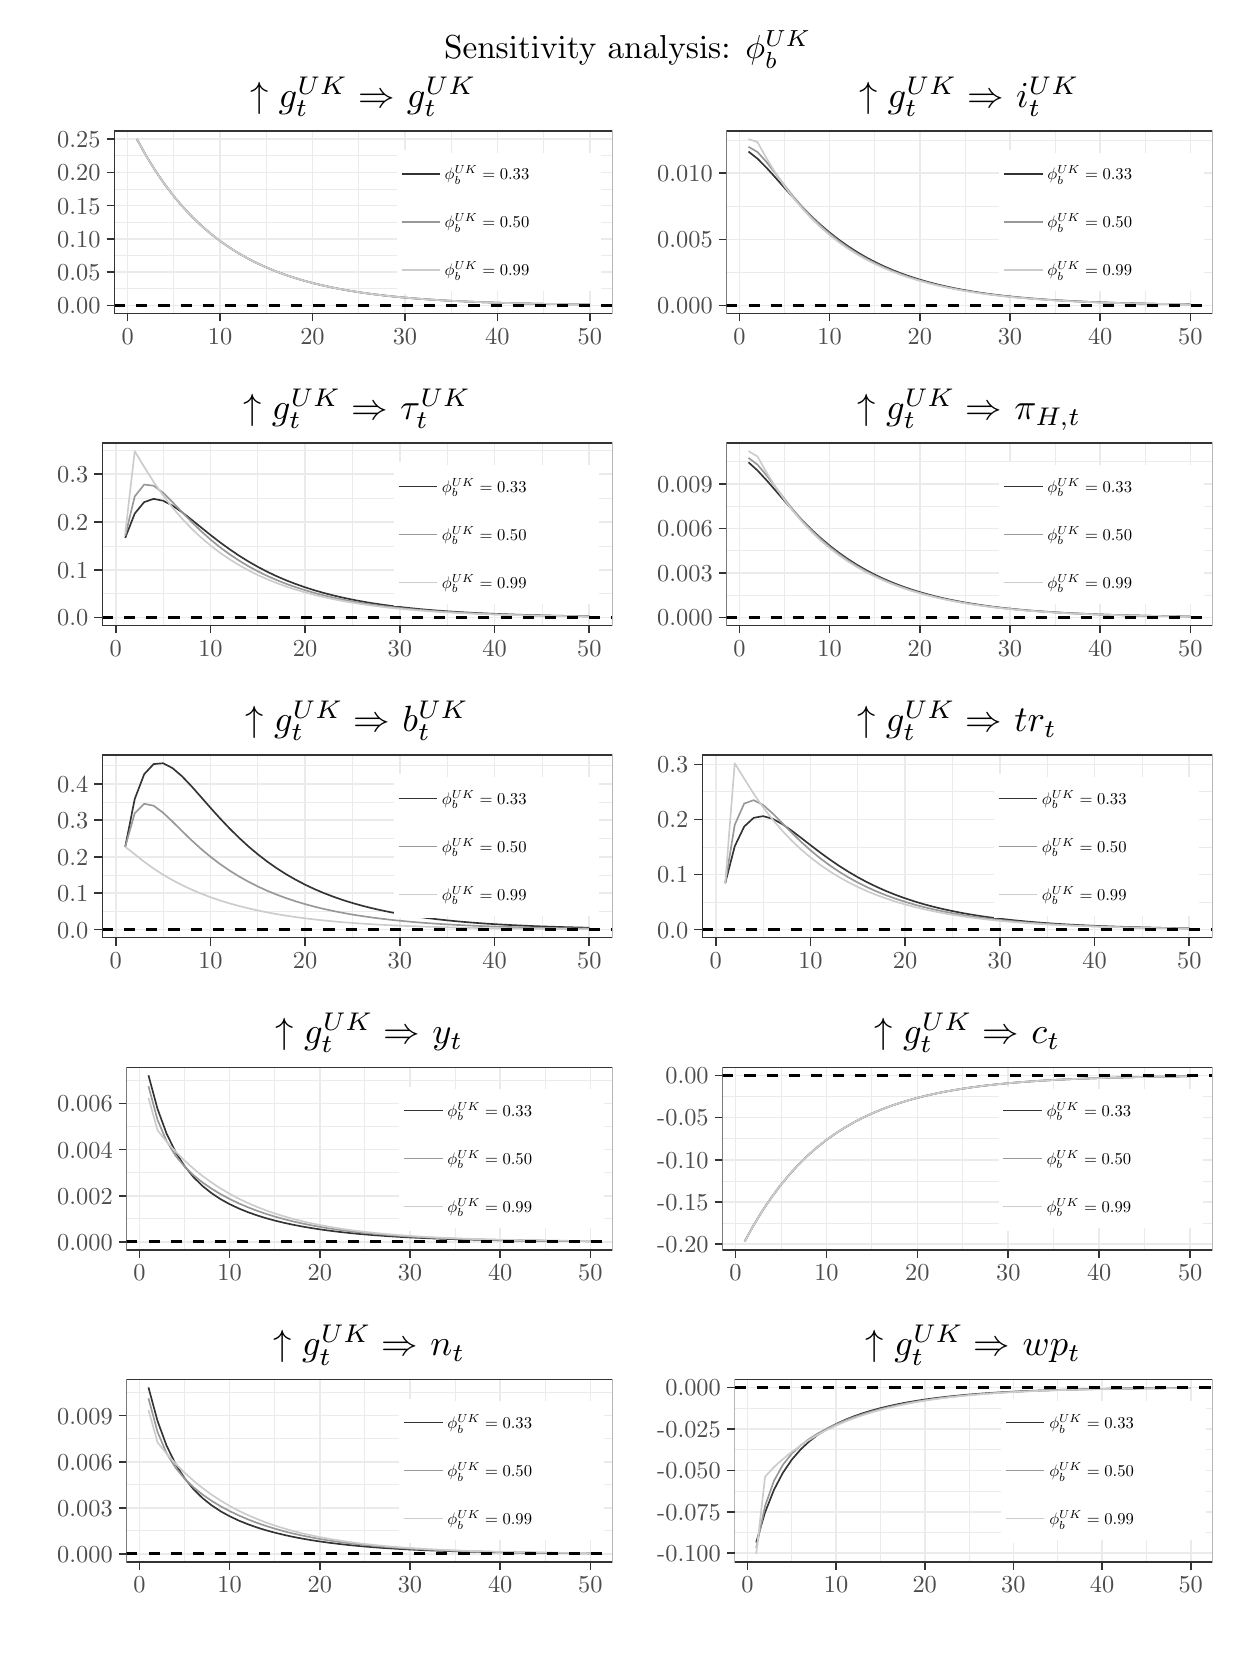
\begin{tikzpicture}[x=1pt,y=1pt]
\definecolor{fillColor}{RGB}{255,255,255}
\path[use as bounding box,fill=fillColor,fill opacity=0.00] (0,0) rectangle (433.62,578.16);
\begin{scope}
\path[clip] (  0.00,451.10) rectangle (216.81,563.87);
\definecolor{drawColor}{RGB}{255,255,255}
\definecolor{fillColor}{RGB}{255,255,255}

\path[draw=drawColor,line width= 0.6pt,line join=round,line cap=round,fill=fillColor] (  0.00,451.10) rectangle (216.81,563.87);
\end{scope}
\begin{scope}
\path[clip] ( 31.27,474.78) rectangle (211.31,540.91);
\definecolor{fillColor}{RGB}{255,255,255}

\path[fill=fillColor] ( 31.27,474.78) rectangle (211.31,540.91);
\definecolor{drawColor}{gray}{0.92}

\path[draw=drawColor,line width= 0.3pt,line join=round] ( 31.27,483.79) --
	(211.31,483.79);

\path[draw=drawColor,line width= 0.3pt,line join=round] ( 31.27,495.82) --
	(211.31,495.82);

\path[draw=drawColor,line width= 0.3pt,line join=round] ( 31.27,507.84) --
	(211.31,507.84);

\path[draw=drawColor,line width= 0.3pt,line join=round] ( 31.27,519.87) --
	(211.31,519.87);

\path[draw=drawColor,line width= 0.3pt,line join=round] ( 31.27,531.89) --
	(211.31,531.89);

\path[draw=drawColor,line width= 0.3pt,line join=round] ( 52.81,474.78) --
	( 52.81,540.91);

\path[draw=drawColor,line width= 0.3pt,line join=round] ( 86.22,474.78) --
	( 86.22,540.91);

\path[draw=drawColor,line width= 0.3pt,line join=round] (119.62,474.78) --
	(119.62,540.91);

\path[draw=drawColor,line width= 0.3pt,line join=round] (153.02,474.78) --
	(153.02,540.91);

\path[draw=drawColor,line width= 0.3pt,line join=round] (186.43,474.78) --
	(186.43,540.91);

\path[draw=drawColor,line width= 0.6pt,line join=round] ( 31.27,477.78) --
	(211.31,477.78);

\path[draw=drawColor,line width= 0.6pt,line join=round] ( 31.27,489.81) --
	(211.31,489.81);

\path[draw=drawColor,line width= 0.6pt,line join=round] ( 31.27,501.83) --
	(211.31,501.83);

\path[draw=drawColor,line width= 0.6pt,line join=round] ( 31.27,513.86) --
	(211.31,513.86);

\path[draw=drawColor,line width= 0.6pt,line join=round] ( 31.27,525.88) --
	(211.31,525.88);

\path[draw=drawColor,line width= 0.6pt,line join=round] ( 31.27,537.90) --
	(211.31,537.90);

\path[draw=drawColor,line width= 0.6pt,line join=round] ( 36.11,474.78) --
	( 36.11,540.91);

\path[draw=drawColor,line width= 0.6pt,line join=round] ( 69.52,474.78) --
	( 69.52,540.91);

\path[draw=drawColor,line width= 0.6pt,line join=round] (102.92,474.78) --
	(102.92,540.91);

\path[draw=drawColor,line width= 0.6pt,line join=round] (136.32,474.78) --
	(136.32,540.91);

\path[draw=drawColor,line width= 0.6pt,line join=round] (169.72,474.78) --
	(169.72,540.91);

\path[draw=drawColor,line width= 0.6pt,line join=round] (203.13,474.78) --
	(203.13,540.91);
\definecolor{drawColor}{gray}{0.20}

\path[draw=drawColor,line width= 0.6pt,line join=round] ( 39.45,537.90) --
	( 42.79,531.89) --
	( 46.13,526.48) --
	( 49.47,521.61) --
	( 52.81,517.23) --
	( 56.15,513.28) --
	( 59.50,509.73) --
	( 62.84,506.54) --
	( 66.18,503.66) --
	( 69.52,501.07) --
	( 72.86,498.75) --
	( 76.20,496.65) --
	( 79.54,494.76) --
	( 82.88,493.06) --
	( 86.22,491.54) --
	( 89.56,490.16) --
	( 92.90,488.92) --
	( 96.24,487.81) --
	( 99.58,486.81) --
	(102.92,485.90) --
	(106.26,485.09) --
	(109.60,484.36) --
	(112.94,483.70) --
	(116.28,483.11) --
	(119.62,482.58) --
	(122.96,482.10) --
	(126.30,481.67) --
	(129.64,481.28) --
	(132.98,480.93) --
	(136.32,480.61) --
	(139.66,480.33) --
	(143.00,480.08) --
	(146.34,479.85) --
	(149.68,479.64) --
	(153.02,479.45) --
	(156.36,479.29) --
	(159.70,479.14) --
	(163.04,479.00) --
	(166.38,478.88) --
	(169.72,478.77) --
	(173.06,478.67) --
	(176.40,478.58) --
	(179.74,478.50) --
	(183.08,478.43) --
	(186.43,478.36) --
	(189.77,478.31) --
	(193.11,478.25) --
	(196.45,478.21) --
	(199.79,478.16) --
	(203.13,478.13);
\definecolor{drawColor}{RGB}{152,152,152}

\path[draw=drawColor,line width= 0.6pt,line join=round] ( 39.45,537.90) --
	( 42.79,531.89) --
	( 46.13,526.48) --
	( 49.47,521.61) --
	( 52.81,517.23) --
	( 56.15,513.28) --
	( 59.50,509.73) --
	( 62.84,506.54) --
	( 66.18,503.66) --
	( 69.52,501.07) --
	( 72.86,498.75) --
	( 76.20,496.65) --
	( 79.54,494.76) --
	( 82.88,493.06) --
	( 86.22,491.54) --
	( 89.56,490.16) --
	( 92.90,488.92) --
	( 96.24,487.81) --
	( 99.58,486.81) --
	(102.92,485.90) --
	(106.26,485.09) --
	(109.60,484.36) --
	(112.94,483.70) --
	(116.28,483.11) --
	(119.62,482.58) --
	(122.96,482.10) --
	(126.30,481.67) --
	(129.64,481.28) --
	(132.98,480.93) --
	(136.32,480.61) --
	(139.66,480.33) --
	(143.00,480.08) --
	(146.34,479.85) --
	(149.68,479.64) --
	(153.02,479.45) --
	(156.36,479.29) --
	(159.70,479.14) --
	(163.04,479.00) --
	(166.38,478.88) --
	(169.72,478.77) --
	(173.06,478.67) --
	(176.40,478.58) --
	(179.74,478.50) --
	(183.08,478.43) --
	(186.43,478.36) --
	(189.77,478.31) --
	(193.11,478.25) --
	(196.45,478.21) --
	(199.79,478.16) --
	(203.13,478.13);
\definecolor{drawColor}{gray}{0.80}

\path[draw=drawColor,line width= 0.6pt,line join=round] ( 39.45,537.90) --
	( 42.79,531.89) --
	( 46.13,526.48) --
	( 49.47,521.61) --
	( 52.81,517.23) --
	( 56.15,513.28) --
	( 59.50,509.73) --
	( 62.84,506.54) --
	( 66.18,503.66) --
	( 69.52,501.07) --
	( 72.86,498.75) --
	( 76.20,496.65) --
	( 79.54,494.76) --
	( 82.88,493.06) --
	( 86.22,491.54) --
	( 89.56,490.16) --
	( 92.90,488.92) --
	( 96.24,487.81) --
	( 99.58,486.81) --
	(102.92,485.90) --
	(106.26,485.09) --
	(109.60,484.36) --
	(112.94,483.70) --
	(116.28,483.11) --
	(119.62,482.58) --
	(122.96,482.10) --
	(126.30,481.67) --
	(129.64,481.28) --
	(132.98,480.93) --
	(136.32,480.61) --
	(139.66,480.33) --
	(143.00,480.08) --
	(146.34,479.85) --
	(149.68,479.64) --
	(153.02,479.45) --
	(156.36,479.29) --
	(159.70,479.14) --
	(163.04,479.00) --
	(166.38,478.88) --
	(169.72,478.77) --
	(173.06,478.67) --
	(176.40,478.58) --
	(179.74,478.50) --
	(183.08,478.43) --
	(186.43,478.36) --
	(189.77,478.31) --
	(193.11,478.25) --
	(196.45,478.21) --
	(199.79,478.16) --
	(203.13,478.13);
\definecolor{drawColor}{RGB}{0,0,0}

\path[draw=drawColor,line width= 1.1pt,dash pattern=on 4pt off 4pt ,line join=round] ( 31.27,477.78) -- (211.31,477.78);
\definecolor{drawColor}{gray}{0.20}

\path[draw=drawColor,line width= 0.6pt,line join=round,line cap=round] ( 31.27,474.78) rectangle (211.31,540.91);
\end{scope}
\begin{scope}
\path[clip] (  0.00,  0.00) rectangle (433.62,578.16);
\definecolor{drawColor}{gray}{0.30}

\node[text=drawColor,anchor=base east,inner sep=0pt, outer sep=0pt, scale=  0.88] at ( 26.32,474.75) {0.00};

\node[text=drawColor,anchor=base east,inner sep=0pt, outer sep=0pt, scale=  0.88] at ( 26.32,486.78) {0.05};

\node[text=drawColor,anchor=base east,inner sep=0pt, outer sep=0pt, scale=  0.88] at ( 26.32,498.80) {0.10};

\node[text=drawColor,anchor=base east,inner sep=0pt, outer sep=0pt, scale=  0.88] at ( 26.32,510.83) {0.15};

\node[text=drawColor,anchor=base east,inner sep=0pt, outer sep=0pt, scale=  0.88] at ( 26.32,522.85) {0.20};

\node[text=drawColor,anchor=base east,inner sep=0pt, outer sep=0pt, scale=  0.88] at ( 26.32,534.87) {0.25};
\end{scope}
\begin{scope}
\path[clip] (  0.00,  0.00) rectangle (433.62,578.16);
\definecolor{drawColor}{gray}{0.20}

\path[draw=drawColor,line width= 0.6pt,line join=round] ( 28.52,477.78) --
	( 31.27,477.78);

\path[draw=drawColor,line width= 0.6pt,line join=round] ( 28.52,489.81) --
	( 31.27,489.81);

\path[draw=drawColor,line width= 0.6pt,line join=round] ( 28.52,501.83) --
	( 31.27,501.83);

\path[draw=drawColor,line width= 0.6pt,line join=round] ( 28.52,513.86) --
	( 31.27,513.86);

\path[draw=drawColor,line width= 0.6pt,line join=round] ( 28.52,525.88) --
	( 31.27,525.88);

\path[draw=drawColor,line width= 0.6pt,line join=round] ( 28.52,537.90) --
	( 31.27,537.90);
\end{scope}
\begin{scope}
\path[clip] (  0.00,  0.00) rectangle (433.62,578.16);
\definecolor{drawColor}{gray}{0.20}

\path[draw=drawColor,line width= 0.6pt,line join=round] ( 36.11,472.03) --
	( 36.11,474.78);

\path[draw=drawColor,line width= 0.6pt,line join=round] ( 69.52,472.03) --
	( 69.52,474.78);

\path[draw=drawColor,line width= 0.6pt,line join=round] (102.92,472.03) --
	(102.92,474.78);

\path[draw=drawColor,line width= 0.6pt,line join=round] (136.32,472.03) --
	(136.32,474.78);

\path[draw=drawColor,line width= 0.6pt,line join=round] (169.72,472.03) --
	(169.72,474.78);

\path[draw=drawColor,line width= 0.6pt,line join=round] (203.13,472.03) --
	(203.13,474.78);
\end{scope}
\begin{scope}
\path[clip] (  0.00,  0.00) rectangle (433.62,578.16);
\definecolor{drawColor}{gray}{0.30}

\node[text=drawColor,anchor=base,inner sep=0pt, outer sep=0pt, scale=  0.88] at ( 36.11,463.76) {0};

\node[text=drawColor,anchor=base,inner sep=0pt, outer sep=0pt, scale=  0.88] at ( 69.52,463.76) {10};

\node[text=drawColor,anchor=base,inner sep=0pt, outer sep=0pt, scale=  0.88] at (102.92,463.76) {20};

\node[text=drawColor,anchor=base,inner sep=0pt, outer sep=0pt, scale=  0.88] at (136.32,463.76) {30};

\node[text=drawColor,anchor=base,inner sep=0pt, outer sep=0pt, scale=  0.88] at (169.72,463.76) {40};

\node[text=drawColor,anchor=base,inner sep=0pt, outer sep=0pt, scale=  0.88] at (203.13,463.76) {50};
\end{scope}
\begin{scope}
\path[clip] (  0.00,  0.00) rectangle (433.62,578.16);
\definecolor{fillColor}{RGB}{255,255,255}

\path[fill=fillColor] (134.34,482.83) rectangle (207.26,532.86);
\end{scope}
\begin{scope}
\path[clip] (  0.00,  0.00) rectangle (433.62,578.16);
\definecolor{fillColor}{RGB}{255,255,255}

\path[fill=fillColor] (133.34,516.52) rectangle (150.69,533.86);
\end{scope}
\begin{scope}
\path[clip] (  0.00,  0.00) rectangle (433.62,578.16);
\definecolor{drawColor}{gray}{0.20}

\path[draw=drawColor,line width= 0.6pt,line join=round] (135.08,525.19) -- (148.95,525.19);
\end{scope}
\begin{scope}
\path[clip] (  0.00,  0.00) rectangle (433.62,578.16);
\definecolor{drawColor}{gray}{0.20}

\path[draw=drawColor,line width= 0.6pt,line join=round] (135.08,525.19) -- (148.95,525.19);
\end{scope}
\begin{scope}
\path[clip] (  0.00,  0.00) rectangle (433.62,578.16);
\definecolor{drawColor}{gray}{0.20}

\path[draw=drawColor,line width= 0.6pt,line join=round] (135.08,525.19) -- (148.95,525.19);
\end{scope}
\begin{scope}
\path[clip] (  0.00,  0.00) rectangle (433.62,578.16);
\definecolor{fillColor}{RGB}{255,255,255}

\path[fill=fillColor] (133.34,499.17) rectangle (150.69,516.52);
\end{scope}
\begin{scope}
\path[clip] (  0.00,  0.00) rectangle (433.62,578.16);
\definecolor{drawColor}{RGB}{152,152,152}

\path[draw=drawColor,line width= 0.6pt,line join=round] (135.08,507.84) -- (148.95,507.84);
\end{scope}
\begin{scope}
\path[clip] (  0.00,  0.00) rectangle (433.62,578.16);
\definecolor{drawColor}{RGB}{152,152,152}

\path[draw=drawColor,line width= 0.6pt,line join=round] (135.08,507.84) -- (148.95,507.84);
\end{scope}
\begin{scope}
\path[clip] (  0.00,  0.00) rectangle (433.62,578.16);
\definecolor{drawColor}{RGB}{152,152,152}

\path[draw=drawColor,line width= 0.6pt,line join=round] (135.08,507.84) -- (148.95,507.84);
\end{scope}
\begin{scope}
\path[clip] (  0.00,  0.00) rectangle (433.62,578.16);
\definecolor{fillColor}{RGB}{255,255,255}

\path[fill=fillColor] (133.34,481.83) rectangle (150.69,499.17);
\end{scope}
\begin{scope}
\path[clip] (  0.00,  0.00) rectangle (433.62,578.16);
\definecolor{drawColor}{gray}{0.80}

\path[draw=drawColor,line width= 0.6pt,line join=round] (135.08,490.50) -- (148.95,490.50);
\end{scope}
\begin{scope}
\path[clip] (  0.00,  0.00) rectangle (433.62,578.16);
\definecolor{drawColor}{gray}{0.80}

\path[draw=drawColor,line width= 0.6pt,line join=round] (135.08,490.50) -- (148.95,490.50);
\end{scope}
\begin{scope}
\path[clip] (  0.00,  0.00) rectangle (433.62,578.16);
\definecolor{drawColor}{gray}{0.80}

\path[draw=drawColor,line width= 0.6pt,line join=round] (135.08,490.50) -- (148.95,490.50);
\end{scope}
\begin{scope}
\path[clip] (  0.00,  0.00) rectangle (433.62,578.16);
\definecolor{drawColor}{RGB}{0,0,0}

\node[text=drawColor,anchor=base west,inner sep=0pt, outer sep=0pt, scale=  0.60] at (150.69,523.12) {${\phi_b^{UK}}=0.33$};
\end{scope}
\begin{scope}
\path[clip] (  0.00,  0.00) rectangle (433.62,578.16);
\definecolor{drawColor}{RGB}{0,0,0}

\node[text=drawColor,anchor=base west,inner sep=0pt, outer sep=0pt, scale=  0.60] at (150.69,505.78) {${\phi_b^{UK}}=0.50$};
\end{scope}
\begin{scope}
\path[clip] (  0.00,  0.00) rectangle (433.62,578.16);
\definecolor{drawColor}{RGB}{0,0,0}

\node[text=drawColor,anchor=base west,inner sep=0pt, outer sep=0pt, scale=  0.60] at (150.69,488.43) {${\phi_b^{UK}}=0.99$};
\end{scope}
\begin{scope}
\path[clip] (  0.00,  0.00) rectangle (433.62,578.16);
\definecolor{drawColor}{RGB}{0,0,0}

\node[text=drawColor,anchor=base,inner sep=0pt, outer sep=0pt, scale=  1.32] at (121.29,549.28) {$\uparrow  g^{UK}_t \Rightarrow $ ${g^{UK}_t}$};
\end{scope}
\begin{scope}
\path[clip] (216.81,451.10) rectangle (433.62,563.87);
\definecolor{drawColor}{RGB}{255,255,255}
\definecolor{fillColor}{RGB}{255,255,255}

\path[draw=drawColor,line width= 0.6pt,line join=round,line cap=round,fill=fillColor] (216.81,451.10) rectangle (433.62,563.87);
\end{scope}
\begin{scope}
\path[clip] (252.48,474.78) rectangle (428.12,540.91);
\definecolor{fillColor}{RGB}{255,255,255}

\path[fill=fillColor] (252.48,474.78) rectangle (428.12,540.91);
\definecolor{drawColor}{gray}{0.92}

\path[draw=drawColor,line width= 0.3pt,line join=round] (252.48,489.72) --
	(428.12,489.72);

\path[draw=drawColor,line width= 0.3pt,line join=round] (252.48,513.58) --
	(428.12,513.58);

\path[draw=drawColor,line width= 0.3pt,line join=round] (252.48,537.45) --
	(428.12,537.45);

\path[draw=drawColor,line width= 0.3pt,line join=round] (273.50,474.78) --
	(273.50,540.91);

\path[draw=drawColor,line width= 0.3pt,line join=round] (306.08,474.78) --
	(306.08,540.91);

\path[draw=drawColor,line width= 0.3pt,line join=round] (338.67,474.78) --
	(338.67,540.91);

\path[draw=drawColor,line width= 0.3pt,line join=round] (371.26,474.78) --
	(371.26,540.91);

\path[draw=drawColor,line width= 0.3pt,line join=round] (403.84,474.78) --
	(403.84,540.91);

\path[draw=drawColor,line width= 0.6pt,line join=round] (252.48,477.78) --
	(428.12,477.78);

\path[draw=drawColor,line width= 0.6pt,line join=round] (252.48,501.65) --
	(428.12,501.65);

\path[draw=drawColor,line width= 0.6pt,line join=round] (252.48,525.52) --
	(428.12,525.52);

\path[draw=drawColor,line width= 0.6pt,line join=round] (257.20,474.78) --
	(257.20,540.91);

\path[draw=drawColor,line width= 0.6pt,line join=round] (289.79,474.78) --
	(289.79,540.91);

\path[draw=drawColor,line width= 0.6pt,line join=round] (322.38,474.78) --
	(322.38,540.91);

\path[draw=drawColor,line width= 0.6pt,line join=round] (354.96,474.78) --
	(354.96,540.91);

\path[draw=drawColor,line width= 0.6pt,line join=round] (387.55,474.78) --
	(387.55,540.91);

\path[draw=drawColor,line width= 0.6pt,line join=round] (420.14,474.78) --
	(420.14,540.91);
\definecolor{drawColor}{gray}{0.20}

\path[draw=drawColor,line width= 0.6pt,line join=round] (260.46,533.39) --
	(263.72,530.82) --
	(266.98,527.54) --
	(270.24,523.94) --
	(273.50,520.25) --
	(276.76,516.63) --
	(280.01,513.17) --
	(283.27,509.92) --
	(286.53,506.90) --
	(289.79,504.12) --
	(293.05,501.58) --
	(296.31,499.26) --
	(299.57,497.15) --
	(302.82,495.24) --
	(306.08,493.51) --
	(309.34,491.95) --
	(312.60,490.54) --
	(315.86,489.27) --
	(319.12,488.13) --
	(322.38,487.10) --
	(325.64,486.17) --
	(328.89,485.33) --
	(332.15,484.58) --
	(335.41,483.90) --
	(338.67,483.29) --
	(341.93,482.74) --
	(345.19,482.24) --
	(348.45,481.79) --
	(351.70,481.39) --
	(354.96,481.03) --
	(358.22,480.71) --
	(361.48,480.41) --
	(364.74,480.15) --
	(368.00,479.91) --
	(371.26,479.70) --
	(374.52,479.51) --
	(377.77,479.34) --
	(381.03,479.18) --
	(384.29,479.04) --
	(387.55,478.92) --
	(390.81,478.80) --
	(394.07,478.70) --
	(397.33,478.61) --
	(400.58,478.53) --
	(403.84,478.45) --
	(407.10,478.38) --
	(410.36,478.32) --
	(413.62,478.27) --
	(416.88,478.22) --
	(420.14,478.18);
\definecolor{drawColor}{RGB}{152,152,152}

\path[draw=drawColor,line width= 0.6pt,line join=round] (260.46,535.11) --
	(263.72,533.22) --
	(266.98,529.61) --
	(270.24,525.41) --
	(273.50,521.14) --
	(276.76,517.05) --
	(280.01,513.25) --
	(283.27,509.77) --
	(286.53,506.60) --
	(289.79,503.74) --
	(293.05,501.15) --
	(296.31,498.82) --
	(299.57,496.71) --
	(302.82,494.82) --
	(306.08,493.12) --
	(309.34,491.59) --
	(312.60,490.20) --
	(315.86,488.96) --
	(319.12,487.84) --
	(322.38,486.84) --
	(325.64,485.93) --
	(328.89,485.12) --
	(332.15,484.38) --
	(335.41,483.72) --
	(338.67,483.13) --
	(341.93,482.59) --
	(345.19,482.11) --
	(348.45,481.68) --
	(351.70,481.29) --
	(354.96,480.94) --
	(358.22,480.62) --
	(361.48,480.34) --
	(364.74,480.08) --
	(368.00,479.85) --
	(371.26,479.65) --
	(374.52,479.46) --
	(377.77,479.29) --
	(381.03,479.14) --
	(384.29,479.01) --
	(387.55,478.88) --
	(390.81,478.77) --
	(394.07,478.67) --
	(397.33,478.58) --
	(400.58,478.50) --
	(403.84,478.43) --
	(407.10,478.37) --
	(410.36,478.31) --
	(413.62,478.26) --
	(416.88,478.21) --
	(420.14,478.17);
\definecolor{drawColor}{gray}{0.80}

\path[draw=drawColor,line width= 0.6pt,line join=round] (260.46,537.90) --
	(263.72,536.79) --
	(266.98,530.94) --
	(270.24,525.62) --
	(273.50,520.84) --
	(276.76,516.53) --
	(280.01,512.66) --
	(283.27,509.17) --
	(286.53,506.03) --
	(289.79,503.21) --
	(293.05,500.66) --
	(296.31,498.37) --
	(299.57,496.32) --
	(302.82,494.46) --
	(306.08,492.79) --
	(309.34,491.29) --
	(312.60,489.94) --
	(315.86,488.73) --
	(319.12,487.63) --
	(322.38,486.65) --
	(325.64,485.76) --
	(328.89,484.96) --
	(332.15,484.24) --
	(335.41,483.60) --
	(338.67,483.02) --
	(341.93,482.49) --
	(345.19,482.02) --
	(348.45,481.60) --
	(351.70,481.22) --
	(354.96,480.87) --
	(358.22,480.56) --
	(361.48,480.29) --
	(364.74,480.04) --
	(368.00,479.81) --
	(371.26,479.61) --
	(374.52,479.42) --
	(377.77,479.26) --
	(381.03,479.11) --
	(384.29,478.98) --
	(387.55,478.86) --
	(390.81,478.75) --
	(394.07,478.65) --
	(397.33,478.57) --
	(400.58,478.49) --
	(403.84,478.42) --
	(407.10,478.35) --
	(410.36,478.30) --
	(413.62,478.25) --
	(416.88,478.20) --
	(420.14,478.16);
\definecolor{drawColor}{RGB}{0,0,0}

\path[draw=drawColor,line width= 1.1pt,dash pattern=on 4pt off 4pt ,line join=round] (252.48,477.78) -- (428.12,477.78);
\definecolor{drawColor}{gray}{0.20}

\path[draw=drawColor,line width= 0.6pt,line join=round,line cap=round] (252.48,474.78) rectangle (428.12,540.91);
\end{scope}
\begin{scope}
\path[clip] (  0.00,  0.00) rectangle (433.62,578.16);
\definecolor{drawColor}{gray}{0.30}

\node[text=drawColor,anchor=base east,inner sep=0pt, outer sep=0pt, scale=  0.88] at (247.53,474.75) {0.000};

\node[text=drawColor,anchor=base east,inner sep=0pt, outer sep=0pt, scale=  0.88] at (247.53,498.62) {0.005};

\node[text=drawColor,anchor=base east,inner sep=0pt, outer sep=0pt, scale=  0.88] at (247.53,522.49) {0.010};
\end{scope}
\begin{scope}
\path[clip] (  0.00,  0.00) rectangle (433.62,578.16);
\definecolor{drawColor}{gray}{0.20}

\path[draw=drawColor,line width= 0.6pt,line join=round] (249.73,477.78) --
	(252.48,477.78);

\path[draw=drawColor,line width= 0.6pt,line join=round] (249.73,501.65) --
	(252.48,501.65);

\path[draw=drawColor,line width= 0.6pt,line join=round] (249.73,525.52) --
	(252.48,525.52);
\end{scope}
\begin{scope}
\path[clip] (  0.00,  0.00) rectangle (433.62,578.16);
\definecolor{drawColor}{gray}{0.20}

\path[draw=drawColor,line width= 0.6pt,line join=round] (257.20,472.03) --
	(257.20,474.78);

\path[draw=drawColor,line width= 0.6pt,line join=round] (289.79,472.03) --
	(289.79,474.78);

\path[draw=drawColor,line width= 0.6pt,line join=round] (322.38,472.03) --
	(322.38,474.78);

\path[draw=drawColor,line width= 0.6pt,line join=round] (354.96,472.03) --
	(354.96,474.78);

\path[draw=drawColor,line width= 0.6pt,line join=round] (387.55,472.03) --
	(387.55,474.78);

\path[draw=drawColor,line width= 0.6pt,line join=round] (420.14,472.03) --
	(420.14,474.78);
\end{scope}
\begin{scope}
\path[clip] (  0.00,  0.00) rectangle (433.62,578.16);
\definecolor{drawColor}{gray}{0.30}

\node[text=drawColor,anchor=base,inner sep=0pt, outer sep=0pt, scale=  0.88] at (257.20,463.76) {0};

\node[text=drawColor,anchor=base,inner sep=0pt, outer sep=0pt, scale=  0.88] at (289.79,463.76) {10};

\node[text=drawColor,anchor=base,inner sep=0pt, outer sep=0pt, scale=  0.88] at (322.38,463.76) {20};

\node[text=drawColor,anchor=base,inner sep=0pt, outer sep=0pt, scale=  0.88] at (354.96,463.76) {30};

\node[text=drawColor,anchor=base,inner sep=0pt, outer sep=0pt, scale=  0.88] at (387.55,463.76) {40};

\node[text=drawColor,anchor=base,inner sep=0pt, outer sep=0pt, scale=  0.88] at (420.14,463.76) {50};
\end{scope}
\begin{scope}
\path[clip] (  0.00,  0.00) rectangle (433.62,578.16);
\definecolor{fillColor}{RGB}{255,255,255}

\path[fill=fillColor] (352.14,482.83) rectangle (425.06,532.86);
\end{scope}
\begin{scope}
\path[clip] (  0.00,  0.00) rectangle (433.62,578.16);
\definecolor{fillColor}{RGB}{255,255,255}

\path[fill=fillColor] (351.14,516.52) rectangle (368.49,533.86);
\end{scope}
\begin{scope}
\path[clip] (  0.00,  0.00) rectangle (433.62,578.16);
\definecolor{drawColor}{gray}{0.20}

\path[draw=drawColor,line width= 0.6pt,line join=round] (352.88,525.19) -- (366.75,525.19);
\end{scope}
\begin{scope}
\path[clip] (  0.00,  0.00) rectangle (433.62,578.16);
\definecolor{drawColor}{gray}{0.20}

\path[draw=drawColor,line width= 0.6pt,line join=round] (352.88,525.19) -- (366.75,525.19);
\end{scope}
\begin{scope}
\path[clip] (  0.00,  0.00) rectangle (433.62,578.16);
\definecolor{drawColor}{gray}{0.20}

\path[draw=drawColor,line width= 0.6pt,line join=round] (352.88,525.19) -- (366.75,525.19);
\end{scope}
\begin{scope}
\path[clip] (  0.00,  0.00) rectangle (433.62,578.16);
\definecolor{fillColor}{RGB}{255,255,255}

\path[fill=fillColor] (351.14,499.17) rectangle (368.49,516.52);
\end{scope}
\begin{scope}
\path[clip] (  0.00,  0.00) rectangle (433.62,578.16);
\definecolor{drawColor}{RGB}{152,152,152}

\path[draw=drawColor,line width= 0.6pt,line join=round] (352.88,507.84) -- (366.75,507.84);
\end{scope}
\begin{scope}
\path[clip] (  0.00,  0.00) rectangle (433.62,578.16);
\definecolor{drawColor}{RGB}{152,152,152}

\path[draw=drawColor,line width= 0.6pt,line join=round] (352.88,507.84) -- (366.75,507.84);
\end{scope}
\begin{scope}
\path[clip] (  0.00,  0.00) rectangle (433.62,578.16);
\definecolor{drawColor}{RGB}{152,152,152}

\path[draw=drawColor,line width= 0.6pt,line join=round] (352.88,507.84) -- (366.75,507.84);
\end{scope}
\begin{scope}
\path[clip] (  0.00,  0.00) rectangle (433.62,578.16);
\definecolor{fillColor}{RGB}{255,255,255}

\path[fill=fillColor] (351.14,481.83) rectangle (368.49,499.17);
\end{scope}
\begin{scope}
\path[clip] (  0.00,  0.00) rectangle (433.62,578.16);
\definecolor{drawColor}{gray}{0.80}

\path[draw=drawColor,line width= 0.6pt,line join=round] (352.88,490.50) -- (366.75,490.50);
\end{scope}
\begin{scope}
\path[clip] (  0.00,  0.00) rectangle (433.62,578.16);
\definecolor{drawColor}{gray}{0.80}

\path[draw=drawColor,line width= 0.6pt,line join=round] (352.88,490.50) -- (366.75,490.50);
\end{scope}
\begin{scope}
\path[clip] (  0.00,  0.00) rectangle (433.62,578.16);
\definecolor{drawColor}{gray}{0.80}

\path[draw=drawColor,line width= 0.6pt,line join=round] (352.88,490.50) -- (366.75,490.50);
\end{scope}
\begin{scope}
\path[clip] (  0.00,  0.00) rectangle (433.62,578.16);
\definecolor{drawColor}{RGB}{0,0,0}

\node[text=drawColor,anchor=base west,inner sep=0pt, outer sep=0pt, scale=  0.60] at (368.49,523.12) {${\phi_b^{UK}}=0.33$};
\end{scope}
\begin{scope}
\path[clip] (  0.00,  0.00) rectangle (433.62,578.16);
\definecolor{drawColor}{RGB}{0,0,0}

\node[text=drawColor,anchor=base west,inner sep=0pt, outer sep=0pt, scale=  0.60] at (368.49,505.78) {${\phi_b^{UK}}=0.50$};
\end{scope}
\begin{scope}
\path[clip] (  0.00,  0.00) rectangle (433.62,578.16);
\definecolor{drawColor}{RGB}{0,0,0}

\node[text=drawColor,anchor=base west,inner sep=0pt, outer sep=0pt, scale=  0.60] at (368.49,488.43) {${\phi_b^{UK}}=0.99$};
\end{scope}
\begin{scope}
\path[clip] (  0.00,  0.00) rectangle (433.62,578.16);
\definecolor{drawColor}{RGB}{0,0,0}

\node[text=drawColor,anchor=base,inner sep=0pt, outer sep=0pt, scale=  1.32] at (340.30,549.28) {$\uparrow  g^{UK}_t \Rightarrow $ ${i^{UK}_t}$};
\end{scope}
\begin{scope}
\path[clip] (  0.00,338.32) rectangle (216.81,451.10);
\definecolor{drawColor}{RGB}{255,255,255}
\definecolor{fillColor}{RGB}{255,255,255}

\path[draw=drawColor,line width= 0.6pt,line join=round,line cap=round,fill=fillColor] (  0.00,338.32) rectangle (216.81,451.10);
\end{scope}
\begin{scope}
\path[clip] ( 26.87,362.00) rectangle (211.31,428.14);
\definecolor{fillColor}{RGB}{255,255,255}

\path[fill=fillColor] ( 26.87,362.00) rectangle (211.31,428.14);
\definecolor{drawColor}{gray}{0.92}

\path[draw=drawColor,line width= 0.3pt,line join=round] ( 26.87,373.63) --
	(211.31,373.63);

\path[draw=drawColor,line width= 0.3pt,line join=round] ( 26.87,390.88) --
	(211.31,390.88);

\path[draw=drawColor,line width= 0.3pt,line join=round] ( 26.87,408.13) --
	(211.31,408.13);

\path[draw=drawColor,line width= 0.3pt,line join=round] ( 26.87,425.38) --
	(211.31,425.38);

\path[draw=drawColor,line width= 0.3pt,line join=round] ( 48.94,362.00) --
	( 48.94,428.14);

\path[draw=drawColor,line width= 0.3pt,line join=round] ( 83.16,362.00) --
	( 83.16,428.14);

\path[draw=drawColor,line width= 0.3pt,line join=round] (117.38,362.00) --
	(117.38,428.14);

\path[draw=drawColor,line width= 0.3pt,line join=round] (151.60,362.00) --
	(151.60,428.14);

\path[draw=drawColor,line width= 0.3pt,line join=round] (185.82,362.00) --
	(185.82,428.14);

\path[draw=drawColor,line width= 0.6pt,line join=round] ( 26.87,365.01) --
	(211.31,365.01);

\path[draw=drawColor,line width= 0.6pt,line join=round] ( 26.87,382.26) --
	(211.31,382.26);

\path[draw=drawColor,line width= 0.6pt,line join=round] ( 26.87,399.51) --
	(211.31,399.51);

\path[draw=drawColor,line width= 0.6pt,line join=round] ( 26.87,416.76) --
	(211.31,416.76);

\path[draw=drawColor,line width= 0.6pt,line join=round] ( 31.83,362.00) --
	( 31.83,428.14);

\path[draw=drawColor,line width= 0.6pt,line join=round] ( 66.05,362.00) --
	( 66.05,428.14);

\path[draw=drawColor,line width= 0.6pt,line join=round] (100.27,362.00) --
	(100.27,428.14);

\path[draw=drawColor,line width= 0.6pt,line join=round] (134.49,362.00) --
	(134.49,428.14);

\path[draw=drawColor,line width= 0.6pt,line join=round] (168.71,362.00) --
	(168.71,428.14);

\path[draw=drawColor,line width= 0.6pt,line join=round] (202.93,362.00) --
	(202.93,428.14);
\definecolor{drawColor}{gray}{0.20}

\path[draw=drawColor,line width= 0.6pt,line join=round] ( 35.25,393.79) --
	( 38.68,402.58) --
	( 42.10,406.72) --
	( 45.52,407.89) --
	( 48.94,407.22) --
	( 52.36,405.44) --
	( 55.79,403.06) --
	( 59.21,400.37) --
	( 62.63,397.60) --
	( 66.05,394.85) --
	( 69.47,392.21) --
	( 72.90,389.73) --
	( 76.32,387.41) --
	( 79.74,385.28) --
	( 83.16,383.33) --
	( 86.58,381.54) --
	( 90.00,379.92) --
	( 93.43,378.45) --
	( 96.85,377.13) --
	(100.27,375.92) --
	(103.69,374.84) --
	(107.11,373.86) --
	(110.54,372.98) --
	(113.96,372.18) --
	(117.38,371.47) --
	(120.80,370.82) --
	(124.22,370.24) --
	(127.65,369.72) --
	(131.07,369.25) --
	(134.49,368.82) --
	(137.91,368.44) --
	(141.33,368.10) --
	(144.75,367.79) --
	(148.18,367.51) --
	(151.60,367.26) --
	(155.02,367.04) --
	(158.44,366.83) --
	(161.86,366.65) --
	(165.29,366.49) --
	(168.71,366.34) --
	(172.13,366.21) --
	(175.55,366.09) --
	(178.97,365.98) --
	(182.40,365.88) --
	(185.82,365.79) --
	(189.24,365.71) --
	(192.66,365.64) --
	(196.08,365.58) --
	(199.50,365.52) --
	(202.93,365.47);
\definecolor{drawColor}{RGB}{152,152,152}

\path[draw=drawColor,line width= 0.6pt,line join=round] ( 35.25,394.53) --
	( 38.68,408.76) --
	( 42.10,413.06) --
	( 45.52,412.64) --
	( 48.94,410.09) --
	( 52.36,406.69) --
	( 55.79,403.09) --
	( 59.21,399.57) --
	( 62.63,396.26) --
	( 66.05,393.20) --
	( 69.47,390.42) --
	( 72.90,387.90) --
	( 76.32,385.62) --
	( 79.74,383.56) --
	( 83.16,381.71) --
	( 86.58,380.04) --
	( 90.00,378.54) --
	( 93.43,377.18) --
	( 96.85,375.97) --
	(100.27,374.87) --
	(103.69,373.88) --
	(107.11,373.00) --
	(110.54,372.20) --
	(113.96,371.48) --
	(117.38,370.83) --
	(120.80,370.25) --
	(124.22,369.72) --
	(127.65,369.25) --
	(131.07,368.83) --
	(134.49,368.45) --
	(137.91,368.10) --
	(141.33,367.79) --
	(144.75,367.51) --
	(148.18,367.26) --
	(151.60,367.04) --
	(155.02,366.84) --
	(158.44,366.65) --
	(161.86,366.49) --
	(165.29,366.34) --
	(168.71,366.21) --
	(172.13,366.09) --
	(175.55,365.98) --
	(178.97,365.88) --
	(182.40,365.79) --
	(185.82,365.72) --
	(189.24,365.64) --
	(192.66,365.58) --
	(196.08,365.52) --
	(199.50,365.47) --
	(202.93,365.43);
\definecolor{drawColor}{gray}{0.80}

\path[draw=drawColor,line width= 0.6pt,line join=round] ( 35.25,395.34) --
	( 38.68,425.13) --
	( 42.10,419.45) --
	( 45.52,414.01) --
	( 48.94,409.11) --
	( 52.36,404.70) --
	( 55.79,400.73) --
	( 59.21,397.16) --
	( 62.63,393.94) --
	( 66.05,391.05) --
	( 69.47,388.44) --
	( 72.90,386.10) --
	( 76.32,383.99) --
	( 79.74,382.09) --
	( 83.16,380.38) --
	( 86.58,378.85) --
	( 90.00,377.46) --
	( 93.43,376.22) --
	( 96.85,375.10) --
	(100.27,374.09) --
	(103.69,373.18) --
	(107.11,372.36) --
	(110.54,371.63) --
	(113.96,370.96) --
	(117.38,370.37) --
	(120.80,369.83) --
	(124.22,369.35) --
	(127.65,368.92) --
	(131.07,368.52) --
	(134.49,368.17) --
	(137.91,367.86) --
	(141.33,367.57) --
	(144.75,367.32) --
	(148.18,367.08) --
	(151.60,366.88) --
	(155.02,366.69) --
	(158.44,366.52) --
	(161.86,366.37) --
	(165.29,366.23) --
	(168.71,366.11) --
	(172.13,366.00) --
	(175.55,365.90) --
	(178.97,365.81) --
	(182.40,365.73) --
	(185.82,365.66) --
	(189.24,365.59) --
	(192.66,365.54) --
	(196.08,365.48) --
	(199.50,365.43) --
	(202.93,365.39);
\definecolor{drawColor}{RGB}{0,0,0}

\path[draw=drawColor,line width= 1.1pt,dash pattern=on 4pt off 4pt ,line join=round] ( 26.87,365.01) -- (211.31,365.01);
\definecolor{drawColor}{gray}{0.20}

\path[draw=drawColor,line width= 0.6pt,line join=round,line cap=round] ( 26.87,362.00) rectangle (211.31,428.14);
\end{scope}
\begin{scope}
\path[clip] (  0.00,  0.00) rectangle (433.62,578.16);
\definecolor{drawColor}{gray}{0.30}

\node[text=drawColor,anchor=base east,inner sep=0pt, outer sep=0pt, scale=  0.88] at ( 21.92,361.98) {0.0};

\node[text=drawColor,anchor=base east,inner sep=0pt, outer sep=0pt, scale=  0.88] at ( 21.92,379.23) {0.1};

\node[text=drawColor,anchor=base east,inner sep=0pt, outer sep=0pt, scale=  0.88] at ( 21.92,396.48) {0.2};

\node[text=drawColor,anchor=base east,inner sep=0pt, outer sep=0pt, scale=  0.88] at ( 21.92,413.73) {0.3};
\end{scope}
\begin{scope}
\path[clip] (  0.00,  0.00) rectangle (433.62,578.16);
\definecolor{drawColor}{gray}{0.20}

\path[draw=drawColor,line width= 0.6pt,line join=round] ( 24.12,365.01) --
	( 26.87,365.01);

\path[draw=drawColor,line width= 0.6pt,line join=round] ( 24.12,382.26) --
	( 26.87,382.26);

\path[draw=drawColor,line width= 0.6pt,line join=round] ( 24.12,399.51) --
	( 26.87,399.51);

\path[draw=drawColor,line width= 0.6pt,line join=round] ( 24.12,416.76) --
	( 26.87,416.76);
\end{scope}
\begin{scope}
\path[clip] (  0.00,  0.00) rectangle (433.62,578.16);
\definecolor{drawColor}{gray}{0.20}

\path[draw=drawColor,line width= 0.6pt,line join=round] ( 31.83,359.25) --
	( 31.83,362.00);

\path[draw=drawColor,line width= 0.6pt,line join=round] ( 66.05,359.25) --
	( 66.05,362.00);

\path[draw=drawColor,line width= 0.6pt,line join=round] (100.27,359.25) --
	(100.27,362.00);

\path[draw=drawColor,line width= 0.6pt,line join=round] (134.49,359.25) --
	(134.49,362.00);

\path[draw=drawColor,line width= 0.6pt,line join=round] (168.71,359.25) --
	(168.71,362.00);

\path[draw=drawColor,line width= 0.6pt,line join=round] (202.93,359.25) --
	(202.93,362.00);
\end{scope}
\begin{scope}
\path[clip] (  0.00,  0.00) rectangle (433.62,578.16);
\definecolor{drawColor}{gray}{0.30}

\node[text=drawColor,anchor=base,inner sep=0pt, outer sep=0pt, scale=  0.88] at ( 31.83,350.99) {0};

\node[text=drawColor,anchor=base,inner sep=0pt, outer sep=0pt, scale=  0.88] at ( 66.05,350.99) {10};

\node[text=drawColor,anchor=base,inner sep=0pt, outer sep=0pt, scale=  0.88] at (100.27,350.99) {20};

\node[text=drawColor,anchor=base,inner sep=0pt, outer sep=0pt, scale=  0.88] at (134.49,350.99) {30};

\node[text=drawColor,anchor=base,inner sep=0pt, outer sep=0pt, scale=  0.88] at (168.71,350.99) {40};

\node[text=drawColor,anchor=base,inner sep=0pt, outer sep=0pt, scale=  0.88] at (202.93,350.99) {50};
\end{scope}
\begin{scope}
\path[clip] (  0.00,  0.00) rectangle (433.62,578.16);
\definecolor{fillColor}{RGB}{255,255,255}

\path[fill=fillColor] (133.35,370.05) rectangle (206.27,420.09);
\end{scope}
\begin{scope}
\path[clip] (  0.00,  0.00) rectangle (433.62,578.16);
\definecolor{fillColor}{RGB}{255,255,255}

\path[fill=fillColor] (132.35,403.74) rectangle (149.70,421.09);
\end{scope}
\begin{scope}
\path[clip] (  0.00,  0.00) rectangle (433.62,578.16);
\definecolor{drawColor}{gray}{0.20}

\path[draw=drawColor,line width= 0.6pt,line join=round] (134.09,412.41) -- (147.96,412.41);
\end{scope}
\begin{scope}
\path[clip] (  0.00,  0.00) rectangle (433.62,578.16);
\definecolor{drawColor}{gray}{0.20}

\path[draw=drawColor,line width= 0.6pt,line join=round] (134.09,412.41) -- (147.96,412.41);
\end{scope}
\begin{scope}
\path[clip] (  0.00,  0.00) rectangle (433.62,578.16);
\definecolor{drawColor}{gray}{0.20}

\path[draw=drawColor,line width= 0.6pt,line join=round] (134.09,412.41) -- (147.96,412.41);
\end{scope}
\begin{scope}
\path[clip] (  0.00,  0.00) rectangle (433.62,578.16);
\definecolor{fillColor}{RGB}{255,255,255}

\path[fill=fillColor] (132.35,386.40) rectangle (149.70,403.74);
\end{scope}
\begin{scope}
\path[clip] (  0.00,  0.00) rectangle (433.62,578.16);
\definecolor{drawColor}{RGB}{152,152,152}

\path[draw=drawColor,line width= 0.6pt,line join=round] (134.09,395.07) -- (147.96,395.07);
\end{scope}
\begin{scope}
\path[clip] (  0.00,  0.00) rectangle (433.62,578.16);
\definecolor{drawColor}{RGB}{152,152,152}

\path[draw=drawColor,line width= 0.6pt,line join=round] (134.09,395.07) -- (147.96,395.07);
\end{scope}
\begin{scope}
\path[clip] (  0.00,  0.00) rectangle (433.62,578.16);
\definecolor{drawColor}{RGB}{152,152,152}

\path[draw=drawColor,line width= 0.6pt,line join=round] (134.09,395.07) -- (147.96,395.07);
\end{scope}
\begin{scope}
\path[clip] (  0.00,  0.00) rectangle (433.62,578.16);
\definecolor{fillColor}{RGB}{255,255,255}

\path[fill=fillColor] (132.35,369.05) rectangle (149.70,386.40);
\end{scope}
\begin{scope}
\path[clip] (  0.00,  0.00) rectangle (433.62,578.16);
\definecolor{drawColor}{gray}{0.80}

\path[draw=drawColor,line width= 0.6pt,line join=round] (134.09,377.72) -- (147.96,377.72);
\end{scope}
\begin{scope}
\path[clip] (  0.00,  0.00) rectangle (433.62,578.16);
\definecolor{drawColor}{gray}{0.80}

\path[draw=drawColor,line width= 0.6pt,line join=round] (134.09,377.72) -- (147.96,377.72);
\end{scope}
\begin{scope}
\path[clip] (  0.00,  0.00) rectangle (433.62,578.16);
\definecolor{drawColor}{gray}{0.80}

\path[draw=drawColor,line width= 0.6pt,line join=round] (134.09,377.72) -- (147.96,377.72);
\end{scope}
\begin{scope}
\path[clip] (  0.00,  0.00) rectangle (433.62,578.16);
\definecolor{drawColor}{RGB}{0,0,0}

\node[text=drawColor,anchor=base west,inner sep=0pt, outer sep=0pt, scale=  0.60] at (149.70,410.35) {${\phi_b^{UK}}=0.33$};
\end{scope}
\begin{scope}
\path[clip] (  0.00,  0.00) rectangle (433.62,578.16);
\definecolor{drawColor}{RGB}{0,0,0}

\node[text=drawColor,anchor=base west,inner sep=0pt, outer sep=0pt, scale=  0.60] at (149.70,393.00) {${\phi_b^{UK}}=0.50$};
\end{scope}
\begin{scope}
\path[clip] (  0.00,  0.00) rectangle (433.62,578.16);
\definecolor{drawColor}{RGB}{0,0,0}

\node[text=drawColor,anchor=base west,inner sep=0pt, outer sep=0pt, scale=  0.60] at (149.70,375.66) {${\phi_b^{UK}}=0.99$};
\end{scope}
\begin{scope}
\path[clip] (  0.00,  0.00) rectangle (433.62,578.16);
\definecolor{drawColor}{RGB}{0,0,0}

\node[text=drawColor,anchor=base,inner sep=0pt, outer sep=0pt, scale=  1.32] at (119.09,436.51) {$\uparrow  g^{UK}_t \Rightarrow $ ${\tau^{UK}_t}$};
\end{scope}
\begin{scope}
\path[clip] (216.81,338.32) rectangle (433.62,451.10);
\definecolor{drawColor}{RGB}{255,255,255}
\definecolor{fillColor}{RGB}{255,255,255}

\path[draw=drawColor,line width= 0.6pt,line join=round,line cap=round,fill=fillColor] (216.81,338.32) rectangle (433.62,451.10);
\end{scope}
\begin{scope}
\path[clip] (252.48,362.00) rectangle (428.12,428.14);
\definecolor{fillColor}{RGB}{255,255,255}

\path[fill=fillColor] (252.48,362.00) rectangle (428.12,428.14);
\definecolor{drawColor}{gray}{0.92}

\path[draw=drawColor,line width= 0.3pt,line join=round] (252.48,373.05) --
	(428.12,373.05);

\path[draw=drawColor,line width= 0.3pt,line join=round] (252.48,389.13) --
	(428.12,389.13);

\path[draw=drawColor,line width= 0.3pt,line join=round] (252.48,405.21) --
	(428.12,405.21);

\path[draw=drawColor,line width= 0.3pt,line join=round] (252.48,421.29) --
	(428.12,421.29);

\path[draw=drawColor,line width= 0.3pt,line join=round] (273.50,362.00) --
	(273.50,428.14);

\path[draw=drawColor,line width= 0.3pt,line join=round] (306.08,362.00) --
	(306.08,428.14);

\path[draw=drawColor,line width= 0.3pt,line join=round] (338.67,362.00) --
	(338.67,428.14);

\path[draw=drawColor,line width= 0.3pt,line join=round] (371.26,362.00) --
	(371.26,428.14);

\path[draw=drawColor,line width= 0.3pt,line join=round] (403.84,362.00) --
	(403.84,428.14);

\path[draw=drawColor,line width= 0.6pt,line join=round] (252.48,365.01) --
	(428.12,365.01);

\path[draw=drawColor,line width= 0.6pt,line join=round] (252.48,381.09) --
	(428.12,381.09);

\path[draw=drawColor,line width= 0.6pt,line join=round] (252.48,397.17) --
	(428.12,397.17);

\path[draw=drawColor,line width= 0.6pt,line join=round] (252.48,413.25) --
	(428.12,413.25);

\path[draw=drawColor,line width= 0.6pt,line join=round] (257.20,362.00) --
	(257.20,428.14);

\path[draw=drawColor,line width= 0.6pt,line join=round] (289.79,362.00) --
	(289.79,428.14);

\path[draw=drawColor,line width= 0.6pt,line join=round] (322.38,362.00) --
	(322.38,428.14);

\path[draw=drawColor,line width= 0.6pt,line join=round] (354.96,362.00) --
	(354.96,428.14);

\path[draw=drawColor,line width= 0.6pt,line join=round] (387.55,362.00) --
	(387.55,428.14);

\path[draw=drawColor,line width= 0.6pt,line join=round] (420.14,362.00) --
	(420.14,428.14);
\definecolor{drawColor}{gray}{0.20}

\path[draw=drawColor,line width= 0.6pt,line join=round] (260.46,421.10) --
	(263.72,418.15) --
	(266.98,414.63) --
	(270.24,410.89) --
	(273.50,407.12) --
	(276.76,403.47) --
	(280.01,400.00) --
	(283.27,396.75) --
	(286.53,393.75) --
	(289.79,391.00) --
	(293.05,388.48) --
	(296.31,386.18) --
	(299.57,384.10) --
	(302.82,382.22) --
	(306.08,380.51) --
	(309.34,378.97) --
	(312.60,377.58) --
	(315.86,376.33) --
	(319.12,375.20) --
	(322.38,374.19) --
	(325.64,373.27) --
	(328.89,372.44) --
	(332.15,371.70) --
	(335.41,371.03) --
	(338.67,370.43) --
	(341.93,369.89) --
	(345.19,369.40) --
	(348.45,368.96) --
	(351.70,368.57) --
	(354.96,368.21) --
	(358.22,367.89) --
	(361.48,367.60) --
	(364.74,367.34) --
	(368.00,367.11) --
	(371.26,366.90) --
	(374.52,366.71) --
	(377.77,366.54) --
	(381.03,366.39) --
	(384.29,366.25) --
	(387.55,366.12) --
	(390.81,366.01) --
	(394.07,365.91) --
	(397.33,365.82) --
	(400.58,365.74) --
	(403.84,365.67) --
	(407.10,365.60) --
	(410.36,365.54) --
	(413.62,365.49) --
	(416.88,365.44) --
	(420.14,365.40);
\definecolor{drawColor}{RGB}{152,152,152}

\path[draw=drawColor,line width= 0.6pt,line join=round] (260.46,422.70) --
	(263.72,420.25) --
	(266.98,416.40) --
	(270.24,412.11) --
	(273.50,407.83) --
	(276.76,403.76) --
	(280.01,399.99) --
	(283.27,396.55) --
	(286.53,393.42) --
	(289.79,390.60) --
	(293.05,388.04) --
	(296.31,385.74) --
	(299.57,383.67) --
	(302.82,381.81) --
	(306.08,380.13) --
	(309.34,378.62) --
	(312.60,377.25) --
	(315.86,376.03) --
	(319.12,374.93) --
	(322.38,373.94) --
	(325.64,373.04) --
	(328.89,372.24) --
	(332.15,371.52) --
	(335.41,370.87) --
	(338.67,370.28) --
	(341.93,369.75) --
	(345.19,369.28) --
	(348.45,368.85) --
	(351.70,368.47) --
	(354.96,368.12) --
	(358.22,367.81) --
	(361.48,367.53) --
	(364.74,367.28) --
	(368.00,367.05) --
	(371.26,366.85) --
	(374.52,366.66) --
	(377.77,366.50) --
	(381.03,366.35) --
	(384.29,366.21) --
	(387.55,366.09) --
	(390.81,365.98) --
	(394.07,365.89) --
	(397.33,365.80) --
	(400.58,365.72) --
	(403.84,365.65) --
	(407.10,365.58) --
	(410.36,365.53) --
	(413.62,365.47) --
	(416.88,365.43) --
	(420.14,365.39);
\definecolor{drawColor}{gray}{0.80}

\path[draw=drawColor,line width= 0.6pt,line join=round] (260.46,425.13) --
	(263.72,423.21) --
	(266.98,417.43) --
	(270.24,412.19) --
	(273.50,407.47) --
	(276.76,403.23) --
	(280.01,399.40) --
	(283.27,395.96) --
	(286.53,392.87) --
	(289.79,390.08) --
	(293.05,387.57) --
	(296.31,385.32) --
	(299.57,383.29) --
	(302.82,381.46) --
	(306.08,379.81) --
	(309.34,378.33) --
	(312.60,377.00) --
	(315.86,375.80) --
	(319.12,374.72) --
	(322.38,373.75) --
	(325.64,372.88) --
	(328.89,372.09) --
	(332.15,371.38) --
	(335.41,370.74) --
	(338.67,370.17) --
	(341.93,369.65) --
	(345.19,369.19) --
	(348.45,368.77) --
	(351.70,368.39) --
	(354.96,368.06) --
	(358.22,367.75) --
	(361.48,367.48) --
	(364.74,367.23) --
	(368.00,367.01) --
	(371.26,366.81) --
	(374.52,366.63) --
	(377.77,366.47) --
	(381.03,366.32) --
	(384.29,366.19) --
	(387.55,366.07) --
	(390.81,365.96) --
	(394.07,365.87) --
	(397.33,365.78) --
	(400.58,365.70) --
	(403.84,365.63) --
	(407.10,365.57) --
	(410.36,365.52) --
	(413.62,365.46) --
	(416.88,365.42) --
	(420.14,365.38);
\definecolor{drawColor}{RGB}{0,0,0}

\path[draw=drawColor,line width= 1.1pt,dash pattern=on 4pt off 4pt ,line join=round] (252.48,365.01) -- (428.12,365.01);
\definecolor{drawColor}{gray}{0.20}

\path[draw=drawColor,line width= 0.6pt,line join=round,line cap=round] (252.48,362.00) rectangle (428.12,428.14);
\end{scope}
\begin{scope}
\path[clip] (  0.00,  0.00) rectangle (433.62,578.16);
\definecolor{drawColor}{gray}{0.30}

\node[text=drawColor,anchor=base east,inner sep=0pt, outer sep=0pt, scale=  0.88] at (247.53,361.98) {0.000};

\node[text=drawColor,anchor=base east,inner sep=0pt, outer sep=0pt, scale=  0.88] at (247.53,378.06) {0.003};

\node[text=drawColor,anchor=base east,inner sep=0pt, outer sep=0pt, scale=  0.88] at (247.53,394.14) {0.006};

\node[text=drawColor,anchor=base east,inner sep=0pt, outer sep=0pt, scale=  0.88] at (247.53,410.22) {0.009};
\end{scope}
\begin{scope}
\path[clip] (  0.00,  0.00) rectangle (433.62,578.16);
\definecolor{drawColor}{gray}{0.20}

\path[draw=drawColor,line width= 0.6pt,line join=round] (249.73,365.01) --
	(252.48,365.01);

\path[draw=drawColor,line width= 0.6pt,line join=round] (249.73,381.09) --
	(252.48,381.09);

\path[draw=drawColor,line width= 0.6pt,line join=round] (249.73,397.17) --
	(252.48,397.17);

\path[draw=drawColor,line width= 0.6pt,line join=round] (249.73,413.25) --
	(252.48,413.25);
\end{scope}
\begin{scope}
\path[clip] (  0.00,  0.00) rectangle (433.62,578.16);
\definecolor{drawColor}{gray}{0.20}

\path[draw=drawColor,line width= 0.6pt,line join=round] (257.20,359.25) --
	(257.20,362.00);

\path[draw=drawColor,line width= 0.6pt,line join=round] (289.79,359.25) --
	(289.79,362.00);

\path[draw=drawColor,line width= 0.6pt,line join=round] (322.38,359.25) --
	(322.38,362.00);

\path[draw=drawColor,line width= 0.6pt,line join=round] (354.96,359.25) --
	(354.96,362.00);

\path[draw=drawColor,line width= 0.6pt,line join=round] (387.55,359.25) --
	(387.55,362.00);

\path[draw=drawColor,line width= 0.6pt,line join=round] (420.14,359.25) --
	(420.14,362.00);
\end{scope}
\begin{scope}
\path[clip] (  0.00,  0.00) rectangle (433.62,578.16);
\definecolor{drawColor}{gray}{0.30}

\node[text=drawColor,anchor=base,inner sep=0pt, outer sep=0pt, scale=  0.88] at (257.20,350.99) {0};

\node[text=drawColor,anchor=base,inner sep=0pt, outer sep=0pt, scale=  0.88] at (289.79,350.99) {10};

\node[text=drawColor,anchor=base,inner sep=0pt, outer sep=0pt, scale=  0.88] at (322.38,350.99) {20};

\node[text=drawColor,anchor=base,inner sep=0pt, outer sep=0pt, scale=  0.88] at (354.96,350.99) {30};

\node[text=drawColor,anchor=base,inner sep=0pt, outer sep=0pt, scale=  0.88] at (387.55,350.99) {40};

\node[text=drawColor,anchor=base,inner sep=0pt, outer sep=0pt, scale=  0.88] at (420.14,350.99) {50};
\end{scope}
\begin{scope}
\path[clip] (  0.00,  0.00) rectangle (433.62,578.16);
\definecolor{fillColor}{RGB}{255,255,255}

\path[fill=fillColor] (352.14,370.05) rectangle (425.06,420.09);
\end{scope}
\begin{scope}
\path[clip] (  0.00,  0.00) rectangle (433.62,578.16);
\definecolor{fillColor}{RGB}{255,255,255}

\path[fill=fillColor] (351.14,403.74) rectangle (368.49,421.09);
\end{scope}
\begin{scope}
\path[clip] (  0.00,  0.00) rectangle (433.62,578.16);
\definecolor{drawColor}{gray}{0.20}

\path[draw=drawColor,line width= 0.6pt,line join=round] (352.88,412.41) -- (366.75,412.41);
\end{scope}
\begin{scope}
\path[clip] (  0.00,  0.00) rectangle (433.62,578.16);
\definecolor{drawColor}{gray}{0.20}

\path[draw=drawColor,line width= 0.6pt,line join=round] (352.88,412.41) -- (366.75,412.41);
\end{scope}
\begin{scope}
\path[clip] (  0.00,  0.00) rectangle (433.62,578.16);
\definecolor{drawColor}{gray}{0.20}

\path[draw=drawColor,line width= 0.6pt,line join=round] (352.88,412.41) -- (366.75,412.41);
\end{scope}
\begin{scope}
\path[clip] (  0.00,  0.00) rectangle (433.62,578.16);
\definecolor{fillColor}{RGB}{255,255,255}

\path[fill=fillColor] (351.14,386.40) rectangle (368.49,403.74);
\end{scope}
\begin{scope}
\path[clip] (  0.00,  0.00) rectangle (433.62,578.16);
\definecolor{drawColor}{RGB}{152,152,152}

\path[draw=drawColor,line width= 0.6pt,line join=round] (352.88,395.07) -- (366.75,395.07);
\end{scope}
\begin{scope}
\path[clip] (  0.00,  0.00) rectangle (433.62,578.16);
\definecolor{drawColor}{RGB}{152,152,152}

\path[draw=drawColor,line width= 0.6pt,line join=round] (352.88,395.07) -- (366.75,395.07);
\end{scope}
\begin{scope}
\path[clip] (  0.00,  0.00) rectangle (433.62,578.16);
\definecolor{drawColor}{RGB}{152,152,152}

\path[draw=drawColor,line width= 0.6pt,line join=round] (352.88,395.07) -- (366.75,395.07);
\end{scope}
\begin{scope}
\path[clip] (  0.00,  0.00) rectangle (433.62,578.16);
\definecolor{fillColor}{RGB}{255,255,255}

\path[fill=fillColor] (351.14,369.05) rectangle (368.49,386.40);
\end{scope}
\begin{scope}
\path[clip] (  0.00,  0.00) rectangle (433.62,578.16);
\definecolor{drawColor}{gray}{0.80}

\path[draw=drawColor,line width= 0.6pt,line join=round] (352.88,377.72) -- (366.75,377.72);
\end{scope}
\begin{scope}
\path[clip] (  0.00,  0.00) rectangle (433.62,578.16);
\definecolor{drawColor}{gray}{0.80}

\path[draw=drawColor,line width= 0.6pt,line join=round] (352.88,377.72) -- (366.75,377.72);
\end{scope}
\begin{scope}
\path[clip] (  0.00,  0.00) rectangle (433.62,578.16);
\definecolor{drawColor}{gray}{0.80}

\path[draw=drawColor,line width= 0.6pt,line join=round] (352.88,377.72) -- (366.75,377.72);
\end{scope}
\begin{scope}
\path[clip] (  0.00,  0.00) rectangle (433.62,578.16);
\definecolor{drawColor}{RGB}{0,0,0}

\node[text=drawColor,anchor=base west,inner sep=0pt, outer sep=0pt, scale=  0.60] at (368.49,410.35) {${\phi_b^{UK}}=0.33$};
\end{scope}
\begin{scope}
\path[clip] (  0.00,  0.00) rectangle (433.62,578.16);
\definecolor{drawColor}{RGB}{0,0,0}

\node[text=drawColor,anchor=base west,inner sep=0pt, outer sep=0pt, scale=  0.60] at (368.49,393.00) {${\phi_b^{UK}}=0.50$};
\end{scope}
\begin{scope}
\path[clip] (  0.00,  0.00) rectangle (433.62,578.16);
\definecolor{drawColor}{RGB}{0,0,0}

\node[text=drawColor,anchor=base west,inner sep=0pt, outer sep=0pt, scale=  0.60] at (368.49,375.66) {${\phi_b^{UK}}=0.99$};
\end{scope}
\begin{scope}
\path[clip] (  0.00,  0.00) rectangle (433.62,578.16);
\definecolor{drawColor}{RGB}{0,0,0}

\node[text=drawColor,anchor=base,inner sep=0pt, outer sep=0pt, scale=  1.32] at (340.30,436.51) {$\uparrow  g^{UK}_t \Rightarrow $ ${\pi_{H,t}}$};
\end{scope}
\begin{scope}
\path[clip] (  0.00,225.55) rectangle (216.81,338.32);
\definecolor{drawColor}{RGB}{255,255,255}
\definecolor{fillColor}{RGB}{255,255,255}

\path[draw=drawColor,line width= 0.6pt,line join=round,line cap=round,fill=fillColor] (  0.00,225.55) rectangle (216.81,338.32);
\end{scope}
\begin{scope}
\path[clip] ( 26.87,249.23) rectangle (211.31,315.36);
\definecolor{fillColor}{RGB}{255,255,255}

\path[fill=fillColor] ( 26.87,249.23) rectangle (211.31,315.36);
\definecolor{drawColor}{gray}{0.92}

\path[draw=drawColor,line width= 0.3pt,line join=round] ( 26.87,258.82) --
	(211.31,258.82);

\path[draw=drawColor,line width= 0.3pt,line join=round] ( 26.87,271.98) --
	(211.31,271.98);

\path[draw=drawColor,line width= 0.3pt,line join=round] ( 26.87,285.15) --
	(211.31,285.15);

\path[draw=drawColor,line width= 0.3pt,line join=round] ( 26.87,298.32) --
	(211.31,298.32);

\path[draw=drawColor,line width= 0.3pt,line join=round] ( 26.87,311.48) --
	(211.31,311.48);

\path[draw=drawColor,line width= 0.3pt,line join=round] ( 48.94,249.23) --
	( 48.94,315.36);

\path[draw=drawColor,line width= 0.3pt,line join=round] ( 83.16,249.23) --
	( 83.16,315.36);

\path[draw=drawColor,line width= 0.3pt,line join=round] (117.38,249.23) --
	(117.38,315.36);

\path[draw=drawColor,line width= 0.3pt,line join=round] (151.60,249.23) --
	(151.60,315.36);

\path[draw=drawColor,line width= 0.3pt,line join=round] (185.82,249.23) --
	(185.82,315.36);

\path[draw=drawColor,line width= 0.6pt,line join=round] ( 26.87,252.23) --
	(211.31,252.23);

\path[draw=drawColor,line width= 0.6pt,line join=round] ( 26.87,265.40) --
	(211.31,265.40);

\path[draw=drawColor,line width= 0.6pt,line join=round] ( 26.87,278.57) --
	(211.31,278.57);

\path[draw=drawColor,line width= 0.6pt,line join=round] ( 26.87,291.73) --
	(211.31,291.73);

\path[draw=drawColor,line width= 0.6pt,line join=round] ( 26.87,304.90) --
	(211.31,304.90);

\path[draw=drawColor,line width= 0.6pt,line join=round] ( 31.83,249.23) --
	( 31.83,315.36);

\path[draw=drawColor,line width= 0.6pt,line join=round] ( 66.05,249.23) --
	( 66.05,315.36);

\path[draw=drawColor,line width= 0.6pt,line join=round] (100.27,249.23) --
	(100.27,315.36);

\path[draw=drawColor,line width= 0.6pt,line join=round] (134.49,249.23) --
	(134.49,315.36);

\path[draw=drawColor,line width= 0.6pt,line join=round] (168.71,249.23) --
	(168.71,315.36);

\path[draw=drawColor,line width= 0.6pt,line join=round] (202.93,249.23) --
	(202.93,315.36);
\definecolor{drawColor}{gray}{0.20}

\path[draw=drawColor,line width= 0.6pt,line join=round] ( 35.25,282.16) --
	( 38.68,299.42) --
	( 42.10,308.40) --
	( 45.52,312.06) --
	( 48.94,312.36) --
	( 52.36,310.59) --
	( 55.79,307.63) --
	( 59.21,304.04) --
	( 62.63,300.17) --
	( 66.05,296.27) --
	( 69.47,292.47) --
	( 72.90,288.85) --
	( 76.32,285.47) --
	( 79.74,282.33) --
	( 83.16,279.45) --
	( 86.58,276.81) --
	( 90.00,274.41) --
	( 93.43,272.23) --
	( 96.85,270.26) --
	(100.27,268.47) --
	(103.69,266.86) --
	(107.11,265.41) --
	(110.54,264.10) --
	(113.96,262.91) --
	(117.38,261.85) --
	(120.80,260.89) --
	(124.22,260.02) --
	(127.65,259.25) --
	(131.07,258.54) --
	(134.49,257.91) --
	(137.91,257.35) --
	(141.33,256.83) --
	(144.75,256.37) --
	(148.18,255.96) --
	(151.60,255.59) --
	(155.02,255.25) --
	(158.44,254.95) --
	(161.86,254.68) --
	(165.29,254.43) --
	(168.71,254.21) --
	(172.13,254.02) --
	(175.55,253.84) --
	(178.97,253.68) --
	(182.40,253.53) --
	(185.82,253.40) --
	(189.24,253.29) --
	(192.66,253.18) --
	(196.08,253.09) --
	(199.50,253.00) --
	(202.93,252.92);
\definecolor{drawColor}{RGB}{152,152,152}

\path[draw=drawColor,line width= 0.6pt,line join=round] ( 35.25,282.16) --
	( 38.68,294.28) --
	( 42.10,297.71) --
	( 45.52,297.01) --
	( 48.94,294.48) --
	( 52.36,291.24) --
	( 55.79,287.84) --
	( 59.21,284.53) --
	( 62.63,281.42) --
	( 66.05,278.57) --
	( 69.47,275.97) --
	( 72.90,273.61) --
	( 76.32,271.48) --
	( 79.74,269.56) --
	( 83.16,267.83) --
	( 86.58,266.27) --
	( 90.00,264.87) --
	( 93.43,263.60) --
	( 96.85,262.47) --
	(100.27,261.44) --
	(103.69,260.52) --
	(107.11,259.69) --
	(110.54,258.95) --
	(113.96,258.28) --
	(117.38,257.67) --
	(120.80,257.13) --
	(124.22,256.64) --
	(127.65,256.20) --
	(131.07,255.80) --
	(134.49,255.44) --
	(137.91,255.12) --
	(141.33,254.83) --
	(144.75,254.57) --
	(148.18,254.34) --
	(151.60,254.13) --
	(155.02,253.94) --
	(158.44,253.77) --
	(161.86,253.62) --
	(165.29,253.48) --
	(168.71,253.35) --
	(172.13,253.24) --
	(175.55,253.14) --
	(178.97,253.05) --
	(182.40,252.97) --
	(185.82,252.89) --
	(189.24,252.83) --
	(192.66,252.77) --
	(196.08,252.71) --
	(199.50,252.67) --
	(202.93,252.62);
\definecolor{drawColor}{gray}{0.80}

\path[draw=drawColor,line width= 0.6pt,line join=round] ( 35.25,282.16) --
	( 38.68,279.47) --
	( 42.10,276.75) --
	( 45.52,274.29) --
	( 48.94,272.09) --
	( 52.36,270.10) --
	( 55.79,268.32) --
	( 59.21,266.71) --
	( 62.63,265.26) --
	( 66.05,263.96) --
	( 69.47,262.78) --
	( 72.90,261.73) --
	( 76.32,260.78) --
	( 79.74,259.93) --
	( 83.16,259.16) --
	( 86.58,258.46) --
	( 90.00,257.84) --
	( 93.43,257.28) --
	( 96.85,256.77) --
	(100.27,256.32) --
	(103.69,255.91) --
	(107.11,255.54) --
	(110.54,255.21) --
	(113.96,254.91) --
	(117.38,254.65) --
	(120.80,254.41) --
	(124.22,254.19) --
	(127.65,253.99) --
	(131.07,253.82) --
	(134.49,253.66) --
	(137.91,253.52) --
	(141.33,253.39) --
	(144.75,253.27) --
	(148.18,253.17) --
	(151.60,253.07) --
	(155.02,252.99) --
	(158.44,252.91) --
	(161.86,252.85) --
	(165.29,252.78) --
	(168.71,252.73) --
	(172.13,252.68) --
	(175.55,252.64) --
	(178.97,252.59) --
	(182.40,252.56) --
	(185.82,252.53) --
	(189.24,252.50) --
	(192.66,252.47) --
	(196.08,252.45) --
	(199.50,252.43) --
	(202.93,252.41);
\definecolor{drawColor}{RGB}{0,0,0}

\path[draw=drawColor,line width= 1.1pt,dash pattern=on 4pt off 4pt ,line join=round] ( 26.87,252.23) -- (211.31,252.23);
\definecolor{drawColor}{gray}{0.20}

\path[draw=drawColor,line width= 0.6pt,line join=round,line cap=round] ( 26.87,249.23) rectangle (211.31,315.36);
\end{scope}
\begin{scope}
\path[clip] (  0.00,  0.00) rectangle (433.62,578.16);
\definecolor{drawColor}{gray}{0.30}

\node[text=drawColor,anchor=base east,inner sep=0pt, outer sep=0pt, scale=  0.88] at ( 21.92,249.20) {0.0};

\node[text=drawColor,anchor=base east,inner sep=0pt, outer sep=0pt, scale=  0.88] at ( 21.92,262.37) {0.1};

\node[text=drawColor,anchor=base east,inner sep=0pt, outer sep=0pt, scale=  0.88] at ( 21.92,275.54) {0.2};

\node[text=drawColor,anchor=base east,inner sep=0pt, outer sep=0pt, scale=  0.88] at ( 21.92,288.70) {0.3};

\node[text=drawColor,anchor=base east,inner sep=0pt, outer sep=0pt, scale=  0.88] at ( 21.92,301.87) {0.4};
\end{scope}
\begin{scope}
\path[clip] (  0.00,  0.00) rectangle (433.62,578.16);
\definecolor{drawColor}{gray}{0.20}

\path[draw=drawColor,line width= 0.6pt,line join=round] ( 24.12,252.23) --
	( 26.87,252.23);

\path[draw=drawColor,line width= 0.6pt,line join=round] ( 24.12,265.40) --
	( 26.87,265.40);

\path[draw=drawColor,line width= 0.6pt,line join=round] ( 24.12,278.57) --
	( 26.87,278.57);

\path[draw=drawColor,line width= 0.6pt,line join=round] ( 24.12,291.73) --
	( 26.87,291.73);

\path[draw=drawColor,line width= 0.6pt,line join=round] ( 24.12,304.90) --
	( 26.87,304.90);
\end{scope}
\begin{scope}
\path[clip] (  0.00,  0.00) rectangle (433.62,578.16);
\definecolor{drawColor}{gray}{0.20}

\path[draw=drawColor,line width= 0.6pt,line join=round] ( 31.83,246.48) --
	( 31.83,249.23);

\path[draw=drawColor,line width= 0.6pt,line join=round] ( 66.05,246.48) --
	( 66.05,249.23);

\path[draw=drawColor,line width= 0.6pt,line join=round] (100.27,246.48) --
	(100.27,249.23);

\path[draw=drawColor,line width= 0.6pt,line join=round] (134.49,246.48) --
	(134.49,249.23);

\path[draw=drawColor,line width= 0.6pt,line join=round] (168.71,246.48) --
	(168.71,249.23);

\path[draw=drawColor,line width= 0.6pt,line join=round] (202.93,246.48) --
	(202.93,249.23);
\end{scope}
\begin{scope}
\path[clip] (  0.00,  0.00) rectangle (433.62,578.16);
\definecolor{drawColor}{gray}{0.30}

\node[text=drawColor,anchor=base,inner sep=0pt, outer sep=0pt, scale=  0.88] at ( 31.83,238.22) {0};

\node[text=drawColor,anchor=base,inner sep=0pt, outer sep=0pt, scale=  0.88] at ( 66.05,238.22) {10};

\node[text=drawColor,anchor=base,inner sep=0pt, outer sep=0pt, scale=  0.88] at (100.27,238.22) {20};

\node[text=drawColor,anchor=base,inner sep=0pt, outer sep=0pt, scale=  0.88] at (134.49,238.22) {30};

\node[text=drawColor,anchor=base,inner sep=0pt, outer sep=0pt, scale=  0.88] at (168.71,238.22) {40};

\node[text=drawColor,anchor=base,inner sep=0pt, outer sep=0pt, scale=  0.88] at (202.93,238.22) {50};
\end{scope}
\begin{scope}
\path[clip] (  0.00,  0.00) rectangle (433.62,578.16);
\definecolor{fillColor}{RGB}{255,255,255}

\path[fill=fillColor] (133.35,257.28) rectangle (206.27,307.31);
\end{scope}
\begin{scope}
\path[clip] (  0.00,  0.00) rectangle (433.62,578.16);
\definecolor{fillColor}{RGB}{255,255,255}

\path[fill=fillColor] (132.35,290.97) rectangle (149.70,308.31);
\end{scope}
\begin{scope}
\path[clip] (  0.00,  0.00) rectangle (433.62,578.16);
\definecolor{drawColor}{gray}{0.20}

\path[draw=drawColor,line width= 0.6pt,line join=round] (134.09,299.64) -- (147.96,299.64);
\end{scope}
\begin{scope}
\path[clip] (  0.00,  0.00) rectangle (433.62,578.16);
\definecolor{drawColor}{gray}{0.20}

\path[draw=drawColor,line width= 0.6pt,line join=round] (134.09,299.64) -- (147.96,299.64);
\end{scope}
\begin{scope}
\path[clip] (  0.00,  0.00) rectangle (433.62,578.16);
\definecolor{drawColor}{gray}{0.20}

\path[draw=drawColor,line width= 0.6pt,line join=round] (134.09,299.64) -- (147.96,299.64);
\end{scope}
\begin{scope}
\path[clip] (  0.00,  0.00) rectangle (433.62,578.16);
\definecolor{fillColor}{RGB}{255,255,255}

\path[fill=fillColor] (132.35,273.62) rectangle (149.70,290.97);
\end{scope}
\begin{scope}
\path[clip] (  0.00,  0.00) rectangle (433.62,578.16);
\definecolor{drawColor}{RGB}{152,152,152}

\path[draw=drawColor,line width= 0.6pt,line join=round] (134.09,282.29) -- (147.96,282.29);
\end{scope}
\begin{scope}
\path[clip] (  0.00,  0.00) rectangle (433.62,578.16);
\definecolor{drawColor}{RGB}{152,152,152}

\path[draw=drawColor,line width= 0.6pt,line join=round] (134.09,282.29) -- (147.96,282.29);
\end{scope}
\begin{scope}
\path[clip] (  0.00,  0.00) rectangle (433.62,578.16);
\definecolor{drawColor}{RGB}{152,152,152}

\path[draw=drawColor,line width= 0.6pt,line join=round] (134.09,282.29) -- (147.96,282.29);
\end{scope}
\begin{scope}
\path[clip] (  0.00,  0.00) rectangle (433.62,578.16);
\definecolor{fillColor}{RGB}{255,255,255}

\path[fill=fillColor] (132.35,256.28) rectangle (149.70,273.62);
\end{scope}
\begin{scope}
\path[clip] (  0.00,  0.00) rectangle (433.62,578.16);
\definecolor{drawColor}{gray}{0.80}

\path[draw=drawColor,line width= 0.6pt,line join=round] (134.09,264.95) -- (147.96,264.95);
\end{scope}
\begin{scope}
\path[clip] (  0.00,  0.00) rectangle (433.62,578.16);
\definecolor{drawColor}{gray}{0.80}

\path[draw=drawColor,line width= 0.6pt,line join=round] (134.09,264.95) -- (147.96,264.95);
\end{scope}
\begin{scope}
\path[clip] (  0.00,  0.00) rectangle (433.62,578.16);
\definecolor{drawColor}{gray}{0.80}

\path[draw=drawColor,line width= 0.6pt,line join=round] (134.09,264.95) -- (147.96,264.95);
\end{scope}
\begin{scope}
\path[clip] (  0.00,  0.00) rectangle (433.62,578.16);
\definecolor{drawColor}{RGB}{0,0,0}

\node[text=drawColor,anchor=base west,inner sep=0pt, outer sep=0pt, scale=  0.60] at (149.70,297.57) {${\phi_b^{UK}}=0.33$};
\end{scope}
\begin{scope}
\path[clip] (  0.00,  0.00) rectangle (433.62,578.16);
\definecolor{drawColor}{RGB}{0,0,0}

\node[text=drawColor,anchor=base west,inner sep=0pt, outer sep=0pt, scale=  0.60] at (149.70,280.23) {${\phi_b^{UK}}=0.50$};
\end{scope}
\begin{scope}
\path[clip] (  0.00,  0.00) rectangle (433.62,578.16);
\definecolor{drawColor}{RGB}{0,0,0}

\node[text=drawColor,anchor=base west,inner sep=0pt, outer sep=0pt, scale=  0.60] at (149.70,262.88) {${\phi_b^{UK}}=0.99$};
\end{scope}
\begin{scope}
\path[clip] (  0.00,  0.00) rectangle (433.62,578.16);
\definecolor{drawColor}{RGB}{0,0,0}

\node[text=drawColor,anchor=base,inner sep=0pt, outer sep=0pt, scale=  1.32] at (119.09,323.73) {$\uparrow  g^{UK}_t \Rightarrow $ ${b^{UK}_t}$};
\end{scope}
\begin{scope}
\path[clip] (216.81,225.55) rectangle (433.62,338.32);
\definecolor{drawColor}{RGB}{255,255,255}
\definecolor{fillColor}{RGB}{255,255,255}

\path[draw=drawColor,line width= 0.6pt,line join=round,line cap=round,fill=fillColor] (216.81,225.55) rectangle (433.62,338.32);
\end{scope}
\begin{scope}
\path[clip] (243.68,249.23) rectangle (428.12,315.36);
\definecolor{fillColor}{RGB}{255,255,255}

\path[fill=fillColor] (243.68,249.23) rectangle (428.12,315.36);
\definecolor{drawColor}{gray}{0.92}

\path[draw=drawColor,line width= 0.3pt,line join=round] (243.68,262.19) --
	(428.12,262.19);

\path[draw=drawColor,line width= 0.3pt,line join=round] (243.68,282.10) --
	(428.12,282.10);

\path[draw=drawColor,line width= 0.3pt,line join=round] (243.68,302.01) --
	(428.12,302.01);

\path[draw=drawColor,line width= 0.3pt,line join=round] (265.75,249.23) --
	(265.75,315.36);

\path[draw=drawColor,line width= 0.3pt,line join=round] (299.97,249.23) --
	(299.97,315.36);

\path[draw=drawColor,line width= 0.3pt,line join=round] (334.19,249.23) --
	(334.19,315.36);

\path[draw=drawColor,line width= 0.3pt,line join=round] (368.41,249.23) --
	(368.41,315.36);

\path[draw=drawColor,line width= 0.3pt,line join=round] (402.63,249.23) --
	(402.63,315.36);

\path[draw=drawColor,line width= 0.6pt,line join=round] (243.68,252.23) --
	(428.12,252.23);

\path[draw=drawColor,line width= 0.6pt,line join=round] (243.68,272.14) --
	(428.12,272.14);

\path[draw=drawColor,line width= 0.6pt,line join=round] (243.68,292.05) --
	(428.12,292.05);

\path[draw=drawColor,line width= 0.6pt,line join=round] (243.68,311.96) --
	(428.12,311.96);

\path[draw=drawColor,line width= 0.6pt,line join=round] (248.64,249.23) --
	(248.64,315.36);

\path[draw=drawColor,line width= 0.6pt,line join=round] (282.86,249.23) --
	(282.86,315.36);

\path[draw=drawColor,line width= 0.6pt,line join=round] (317.08,249.23) --
	(317.08,315.36);

\path[draw=drawColor,line width= 0.6pt,line join=round] (351.30,249.23) --
	(351.30,315.36);

\path[draw=drawColor,line width= 0.6pt,line join=round] (385.52,249.23) --
	(385.52,315.36);

\path[draw=drawColor,line width= 0.6pt,line join=round] (419.74,249.23) --
	(419.74,315.36);
\definecolor{drawColor}{gray}{0.20}

\path[draw=drawColor,line width= 0.6pt,line join=round] (252.06,269.01) --
	(255.49,282.34) --
	(258.91,289.48) --
	(262.33,292.63) --
	(265.75,293.24) --
	(269.17,292.29) --
	(272.60,290.41) --
	(276.02,288.03) --
	(279.44,285.43) --
	(282.86,282.77) --
	(286.28,280.16) --
	(289.71,277.67) --
	(293.13,275.33) --
	(296.55,273.16) --
	(299.97,271.16) --
	(303.39,269.33) --
	(306.81,267.67) --
	(310.24,266.15) --
	(313.66,264.78) --
	(317.08,263.54) --
	(320.50,262.42) --
	(323.92,261.40) --
	(327.35,260.49) --
	(330.77,259.67) --
	(334.19,258.93) --
	(337.61,258.26) --
	(341.03,257.66) --
	(344.46,257.11) --
	(347.88,256.63) --
	(351.30,256.19) --
	(354.72,255.79) --
	(358.14,255.44) --
	(361.56,255.12) --
	(364.99,254.83) --
	(368.41,254.57) --
	(371.83,254.33) --
	(375.25,254.12) --
	(378.67,253.94) --
	(382.10,253.77) --
	(385.52,253.61) --
	(388.94,253.47) --
	(392.36,253.35) --
	(395.78,253.24) --
	(399.21,253.14) --
	(402.63,253.05) --
	(406.05,252.97) --
	(409.47,252.89) --
	(412.89,252.83) --
	(416.31,252.77) --
	(419.74,252.71);
\definecolor{drawColor}{RGB}{152,152,152}

\path[draw=drawColor,line width= 0.6pt,line join=round] (252.06,269.05) --
	(255.49,290.09) --
	(258.91,297.78) --
	(262.33,299.02) --
	(265.75,297.27) --
	(269.17,294.24) --
	(272.60,290.79) --
	(276.02,287.31) --
	(279.44,283.99) --
	(282.86,280.91) --
	(286.28,278.09) --
	(289.71,275.53) --
	(293.13,273.21) --
	(296.55,271.12) --
	(299.97,269.24) --
	(303.39,267.54) --
	(306.81,266.01) --
	(310.24,264.63) --
	(313.66,263.39) --
	(317.08,262.28) --
	(320.50,261.27) --
	(323.92,260.37) --
	(327.35,259.55) --
	(330.77,258.82) --
	(334.19,258.16) --
	(337.61,257.57) --
	(341.03,257.04) --
	(344.46,256.56) --
	(347.88,256.12) --
	(351.30,255.73) --
	(354.72,255.38) --
	(358.14,255.07) --
	(361.56,254.79) --
	(364.99,254.53) --
	(368.41,254.30) --
	(371.83,254.09) --
	(375.25,253.91) --
	(378.67,253.74) --
	(382.10,253.59) --
	(385.52,253.45) --
	(388.94,253.33) --
	(392.36,253.22) --
	(395.78,253.12) --
	(399.21,253.03) --
	(402.63,252.95) --
	(406.05,252.88) --
	(409.47,252.82) --
	(412.89,252.76) --
	(416.31,252.71) --
	(419.74,252.66);
\definecolor{drawColor}{gray}{0.80}

\path[draw=drawColor,line width= 0.6pt,line join=round] (252.06,269.12) --
	(255.49,312.36) --
	(258.91,306.80) --
	(262.33,301.35) --
	(265.75,296.43) --
	(269.17,292.01) --
	(272.60,288.04) --
	(276.02,284.46) --
	(279.44,281.23) --
	(282.86,278.33) --
	(286.28,275.72) --
	(289.71,273.37) --
	(293.13,271.26) --
	(296.55,269.36) --
	(299.97,267.64) --
	(303.39,266.10) --
	(306.81,264.72) --
	(310.24,263.47) --
	(313.66,262.34) --
	(317.08,261.33) --
	(320.50,260.42) --
	(323.92,259.60) --
	(327.35,258.87) --
	(330.77,258.20) --
	(334.19,257.61) --
	(337.61,257.07) --
	(341.03,256.59) --
	(344.46,256.15) --
	(347.88,255.76) --
	(351.30,255.41) --
	(354.72,255.09) --
	(358.14,254.80) --
	(361.56,254.55) --
	(364.99,254.31) --
	(368.41,254.11) --
	(371.83,253.92) --
	(375.25,253.75) --
	(378.67,253.60) --
	(382.10,253.46) --
	(385.52,253.34) --
	(388.94,253.23) --
	(392.36,253.13) --
	(395.78,253.04) --
	(399.21,252.96) --
	(402.63,252.89) --
	(406.05,252.82) --
	(409.47,252.76) --
	(412.89,252.71) --
	(416.31,252.66) --
	(419.74,252.62);
\definecolor{drawColor}{RGB}{0,0,0}

\path[draw=drawColor,line width= 1.1pt,dash pattern=on 4pt off 4pt ,line join=round] (243.68,252.23) -- (428.12,252.23);
\definecolor{drawColor}{gray}{0.20}

\path[draw=drawColor,line width= 0.6pt,line join=round,line cap=round] (243.68,249.23) rectangle (428.12,315.36);
\end{scope}
\begin{scope}
\path[clip] (  0.00,  0.00) rectangle (433.62,578.16);
\definecolor{drawColor}{gray}{0.30}

\node[text=drawColor,anchor=base east,inner sep=0pt, outer sep=0pt, scale=  0.88] at (238.73,249.20) {0.0};

\node[text=drawColor,anchor=base east,inner sep=0pt, outer sep=0pt, scale=  0.88] at (238.73,269.11) {0.1};

\node[text=drawColor,anchor=base east,inner sep=0pt, outer sep=0pt, scale=  0.88] at (238.73,289.02) {0.2};

\node[text=drawColor,anchor=base east,inner sep=0pt, outer sep=0pt, scale=  0.88] at (238.73,308.93) {0.3};
\end{scope}
\begin{scope}
\path[clip] (  0.00,  0.00) rectangle (433.62,578.16);
\definecolor{drawColor}{gray}{0.20}

\path[draw=drawColor,line width= 0.6pt,line join=round] (240.93,252.23) --
	(243.68,252.23);

\path[draw=drawColor,line width= 0.6pt,line join=round] (240.93,272.14) --
	(243.68,272.14);

\path[draw=drawColor,line width= 0.6pt,line join=round] (240.93,292.05) --
	(243.68,292.05);

\path[draw=drawColor,line width= 0.6pt,line join=round] (240.93,311.96) --
	(243.68,311.96);
\end{scope}
\begin{scope}
\path[clip] (  0.00,  0.00) rectangle (433.62,578.16);
\definecolor{drawColor}{gray}{0.20}

\path[draw=drawColor,line width= 0.6pt,line join=round] (248.64,246.48) --
	(248.64,249.23);

\path[draw=drawColor,line width= 0.6pt,line join=round] (282.86,246.48) --
	(282.86,249.23);

\path[draw=drawColor,line width= 0.6pt,line join=round] (317.08,246.48) --
	(317.08,249.23);

\path[draw=drawColor,line width= 0.6pt,line join=round] (351.30,246.48) --
	(351.30,249.23);

\path[draw=drawColor,line width= 0.6pt,line join=round] (385.52,246.48) --
	(385.52,249.23);

\path[draw=drawColor,line width= 0.6pt,line join=round] (419.74,246.48) --
	(419.74,249.23);
\end{scope}
\begin{scope}
\path[clip] (  0.00,  0.00) rectangle (433.62,578.16);
\definecolor{drawColor}{gray}{0.30}

\node[text=drawColor,anchor=base,inner sep=0pt, outer sep=0pt, scale=  0.88] at (248.64,238.22) {0};

\node[text=drawColor,anchor=base,inner sep=0pt, outer sep=0pt, scale=  0.88] at (282.86,238.22) {10};

\node[text=drawColor,anchor=base,inner sep=0pt, outer sep=0pt, scale=  0.88] at (317.08,238.22) {20};

\node[text=drawColor,anchor=base,inner sep=0pt, outer sep=0pt, scale=  0.88] at (351.30,238.22) {30};

\node[text=drawColor,anchor=base,inner sep=0pt, outer sep=0pt, scale=  0.88] at (385.52,238.22) {40};

\node[text=drawColor,anchor=base,inner sep=0pt, outer sep=0pt, scale=  0.88] at (419.74,238.22) {50};
\end{scope}
\begin{scope}
\path[clip] (  0.00,  0.00) rectangle (433.62,578.16);
\definecolor{fillColor}{RGB}{255,255,255}

\path[fill=fillColor] (350.16,257.28) rectangle (423.08,307.31);
\end{scope}
\begin{scope}
\path[clip] (  0.00,  0.00) rectangle (433.62,578.16);
\definecolor{fillColor}{RGB}{255,255,255}

\path[fill=fillColor] (349.16,290.97) rectangle (366.51,308.31);
\end{scope}
\begin{scope}
\path[clip] (  0.00,  0.00) rectangle (433.62,578.16);
\definecolor{drawColor}{gray}{0.20}

\path[draw=drawColor,line width= 0.6pt,line join=round] (350.90,299.64) -- (364.77,299.64);
\end{scope}
\begin{scope}
\path[clip] (  0.00,  0.00) rectangle (433.62,578.16);
\definecolor{drawColor}{gray}{0.20}

\path[draw=drawColor,line width= 0.6pt,line join=round] (350.90,299.64) -- (364.77,299.64);
\end{scope}
\begin{scope}
\path[clip] (  0.00,  0.00) rectangle (433.62,578.16);
\definecolor{drawColor}{gray}{0.20}

\path[draw=drawColor,line width= 0.6pt,line join=round] (350.90,299.64) -- (364.77,299.64);
\end{scope}
\begin{scope}
\path[clip] (  0.00,  0.00) rectangle (433.62,578.16);
\definecolor{fillColor}{RGB}{255,255,255}

\path[fill=fillColor] (349.16,273.62) rectangle (366.51,290.97);
\end{scope}
\begin{scope}
\path[clip] (  0.00,  0.00) rectangle (433.62,578.16);
\definecolor{drawColor}{RGB}{152,152,152}

\path[draw=drawColor,line width= 0.6pt,line join=round] (350.90,282.29) -- (364.77,282.29);
\end{scope}
\begin{scope}
\path[clip] (  0.00,  0.00) rectangle (433.62,578.16);
\definecolor{drawColor}{RGB}{152,152,152}

\path[draw=drawColor,line width= 0.6pt,line join=round] (350.90,282.29) -- (364.77,282.29);
\end{scope}
\begin{scope}
\path[clip] (  0.00,  0.00) rectangle (433.62,578.16);
\definecolor{drawColor}{RGB}{152,152,152}

\path[draw=drawColor,line width= 0.6pt,line join=round] (350.90,282.29) -- (364.77,282.29);
\end{scope}
\begin{scope}
\path[clip] (  0.00,  0.00) rectangle (433.62,578.16);
\definecolor{fillColor}{RGB}{255,255,255}

\path[fill=fillColor] (349.16,256.28) rectangle (366.51,273.62);
\end{scope}
\begin{scope}
\path[clip] (  0.00,  0.00) rectangle (433.62,578.16);
\definecolor{drawColor}{gray}{0.80}

\path[draw=drawColor,line width= 0.6pt,line join=round] (350.90,264.95) -- (364.77,264.95);
\end{scope}
\begin{scope}
\path[clip] (  0.00,  0.00) rectangle (433.62,578.16);
\definecolor{drawColor}{gray}{0.80}

\path[draw=drawColor,line width= 0.6pt,line join=round] (350.90,264.95) -- (364.77,264.95);
\end{scope}
\begin{scope}
\path[clip] (  0.00,  0.00) rectangle (433.62,578.16);
\definecolor{drawColor}{gray}{0.80}

\path[draw=drawColor,line width= 0.6pt,line join=round] (350.90,264.95) -- (364.77,264.95);
\end{scope}
\begin{scope}
\path[clip] (  0.00,  0.00) rectangle (433.62,578.16);
\definecolor{drawColor}{RGB}{0,0,0}

\node[text=drawColor,anchor=base west,inner sep=0pt, outer sep=0pt, scale=  0.60] at (366.51,297.57) {${\phi_b^{UK}}=0.33$};
\end{scope}
\begin{scope}
\path[clip] (  0.00,  0.00) rectangle (433.62,578.16);
\definecolor{drawColor}{RGB}{0,0,0}

\node[text=drawColor,anchor=base west,inner sep=0pt, outer sep=0pt, scale=  0.60] at (366.51,280.23) {${\phi_b^{UK}}=0.50$};
\end{scope}
\begin{scope}
\path[clip] (  0.00,  0.00) rectangle (433.62,578.16);
\definecolor{drawColor}{RGB}{0,0,0}

\node[text=drawColor,anchor=base west,inner sep=0pt, outer sep=0pt, scale=  0.60] at (366.51,262.88) {${\phi_b^{UK}}=0.99$};
\end{scope}
\begin{scope}
\path[clip] (  0.00,  0.00) rectangle (433.62,578.16);
\definecolor{drawColor}{RGB}{0,0,0}

\node[text=drawColor,anchor=base,inner sep=0pt, outer sep=0pt, scale=  1.32] at (335.90,323.73) {$\uparrow  g^{UK}_t \Rightarrow $ ${tr_t}$};
\end{scope}
\begin{scope}
\path[clip] (  0.00,112.77) rectangle (216.81,225.55);
\definecolor{drawColor}{RGB}{255,255,255}
\definecolor{fillColor}{RGB}{255,255,255}

\path[draw=drawColor,line width= 0.6pt,line join=round,line cap=round,fill=fillColor] (  0.00,112.77) rectangle (216.81,225.55);
\end{scope}
\begin{scope}
\path[clip] ( 35.67,136.45) rectangle (211.31,202.59);
\definecolor{fillColor}{RGB}{255,255,255}

\path[fill=fillColor] ( 35.67,136.45) rectangle (211.31,202.59);
\definecolor{drawColor}{gray}{0.92}

\path[draw=drawColor,line width= 0.3pt,line join=round] ( 35.67,147.78) --
	(211.31,147.78);

\path[draw=drawColor,line width= 0.3pt,line join=round] ( 35.67,164.42) --
	(211.31,164.42);

\path[draw=drawColor,line width= 0.3pt,line join=round] ( 35.67,181.06) --
	(211.31,181.06);

\path[draw=drawColor,line width= 0.3pt,line join=round] ( 35.67,197.71) --
	(211.31,197.71);

\path[draw=drawColor,line width= 0.3pt,line join=round] ( 56.69,136.45) --
	( 56.69,202.59);

\path[draw=drawColor,line width= 0.3pt,line join=round] ( 89.27,136.45) --
	( 89.27,202.59);

\path[draw=drawColor,line width= 0.3pt,line join=round] (121.86,136.45) --
	(121.86,202.59);

\path[draw=drawColor,line width= 0.3pt,line join=round] (154.45,136.45) --
	(154.45,202.59);

\path[draw=drawColor,line width= 0.3pt,line join=round] (187.03,136.45) --
	(187.03,202.59);

\path[draw=drawColor,line width= 0.6pt,line join=round] ( 35.67,139.46) --
	(211.31,139.46);

\path[draw=drawColor,line width= 0.6pt,line join=round] ( 35.67,156.10) --
	(211.31,156.10);

\path[draw=drawColor,line width= 0.6pt,line join=round] ( 35.67,172.74) --
	(211.31,172.74);

\path[draw=drawColor,line width= 0.6pt,line join=round] ( 35.67,189.39) --
	(211.31,189.39);

\path[draw=drawColor,line width= 0.6pt,line join=round] ( 40.39,136.45) --
	( 40.39,202.59);

\path[draw=drawColor,line width= 0.6pt,line join=round] ( 72.98,136.45) --
	( 72.98,202.59);

\path[draw=drawColor,line width= 0.6pt,line join=round] (105.57,136.45) --
	(105.57,202.59);

\path[draw=drawColor,line width= 0.6pt,line join=round] (138.15,136.45) --
	(138.15,202.59);

\path[draw=drawColor,line width= 0.6pt,line join=round] (170.74,136.45) --
	(170.74,202.59);

\path[draw=drawColor,line width= 0.6pt,line join=round] (203.33,136.45) --
	(203.33,202.59);
\definecolor{drawColor}{gray}{0.20}

\path[draw=drawColor,line width= 0.6pt,line join=round] ( 43.65,199.58) --
	( 46.91,187.50) --
	( 50.17,178.59) --
	( 53.43,171.90) --
	( 56.69,166.78) --
	( 59.95,162.77) --
	( 63.20,159.58) --
	( 66.46,156.99) --
	( 69.72,154.84) --
	( 72.98,153.03) --
	( 76.24,151.50) --
	( 79.50,150.17) --
	( 82.76,149.02) --
	( 86.01,148.00) --
	( 89.27,147.11) --
	( 92.53,146.32) --
	( 95.79,145.62) --
	( 99.05,144.99) --
	(102.31,144.43) --
	(105.57,143.93) --
	(108.83,143.48) --
	(112.08,143.07) --
	(115.34,142.71) --
	(118.60,142.38) --
	(121.86,142.09) --
	(125.12,141.83) --
	(128.38,141.59) --
	(131.64,141.38) --
	(134.89,141.18) --
	(138.15,141.01) --
	(141.41,140.86) --
	(144.67,140.72) --
	(147.93,140.59) --
	(151.19,140.48) --
	(154.45,140.37) --
	(157.71,140.28) --
	(160.96,140.20) --
	(164.22,140.13) --
	(167.48,140.06) --
	(170.74,140.00) --
	(174.00,139.95) --
	(177.26,139.90) --
	(180.52,139.85) --
	(183.77,139.81) --
	(187.03,139.78) --
	(190.29,139.75) --
	(193.55,139.72) --
	(196.81,139.69) --
	(200.07,139.67) --
	(203.33,139.65);
\definecolor{drawColor}{RGB}{152,152,152}

\path[draw=drawColor,line width= 0.6pt,line join=round] ( 43.65,195.63) --
	( 46.91,183.54) --
	( 50.17,175.86) --
	( 53.43,170.56) --
	( 56.69,166.62) --
	( 59.95,163.48) --
	( 63.20,160.87) --
	( 66.46,158.62) --
	( 69.72,156.65) --
	( 72.98,154.90) --
	( 76.24,153.34) --
	( 79.50,151.95) --
	( 82.76,150.70) --
	( 86.01,149.57) --
	( 89.27,148.56) --
	( 92.53,147.65) --
	( 95.79,146.83) --
	( 99.05,146.09) --
	(102.31,145.43) --
	(105.57,144.83) --
	(108.83,144.29) --
	(112.08,143.81) --
	(115.34,143.37) --
	(118.60,142.98) --
	(121.86,142.63) --
	(125.12,142.31) --
	(128.38,142.03) --
	(131.64,141.77) --
	(134.89,141.54) --
	(138.15,141.33) --
	(141.41,141.14) --
	(144.67,140.98) --
	(147.93,140.82) --
	(151.19,140.69) --
	(154.45,140.56) --
	(157.71,140.45) --
	(160.96,140.35) --
	(164.22,140.26) --
	(167.48,140.18) --
	(170.74,140.11) --
	(174.00,140.05) --
	(177.26,139.99) --
	(180.52,139.93) --
	(183.77,139.89) --
	(187.03,139.84) --
	(190.29,139.81) --
	(193.55,139.77) --
	(196.81,139.74) --
	(200.07,139.71) --
	(203.33,139.69);
\definecolor{drawColor}{gray}{0.80}

\path[draw=drawColor,line width= 0.6pt,line join=round] ( 43.65,191.46) --
	( 46.91,179.76) --
	( 50.17,175.66) --
	( 53.43,172.04) --
	( 56.69,168.78) --
	( 59.95,165.85) --
	( 63.20,163.21) --
	( 66.46,160.84) --
	( 69.72,158.70) --
	( 72.98,156.78) --
	( 76.24,155.04) --
	( 79.50,153.49) --
	( 82.76,152.08) --
	( 86.01,150.82) --
	( 89.27,149.68) --
	( 92.53,148.66) --
	( 95.79,147.74) --
	( 99.05,146.91) --
	(102.31,146.17) --
	(105.57,145.50) --
	(108.83,144.89) --
	(112.08,144.35) --
	(115.34,143.86) --
	(118.60,143.42) --
	(121.86,143.02) --
	(125.12,142.67) --
	(128.38,142.35) --
	(131.64,142.06) --
	(134.89,141.80) --
	(138.15,141.56) --
	(141.41,141.35) --
	(144.67,141.16) --
	(147.93,140.99) --
	(151.19,140.84) --
	(154.45,140.70) --
	(157.71,140.58) --
	(160.96,140.46) --
	(164.22,140.36) --
	(167.48,140.27) --
	(170.74,140.19) --
	(174.00,140.12) --
	(177.26,140.05) --
	(180.52,139.99) --
	(183.77,139.94) --
	(187.03,139.89) --
	(190.29,139.85) --
	(193.55,139.81) --
	(196.81,139.77) --
	(200.07,139.74) --
	(203.33,139.71);
\definecolor{drawColor}{RGB}{0,0,0}

\path[draw=drawColor,line width= 1.1pt,dash pattern=on 4pt off 4pt ,line join=round] ( 35.67,139.46) -- (211.31,139.46);
\definecolor{drawColor}{gray}{0.20}

\path[draw=drawColor,line width= 0.6pt,line join=round,line cap=round] ( 35.67,136.45) rectangle (211.31,202.59);
\end{scope}
\begin{scope}
\path[clip] (  0.00,  0.00) rectangle (433.62,578.16);
\definecolor{drawColor}{gray}{0.30}

\node[text=drawColor,anchor=base east,inner sep=0pt, outer sep=0pt, scale=  0.88] at ( 30.72,136.43) {0.000};

\node[text=drawColor,anchor=base east,inner sep=0pt, outer sep=0pt, scale=  0.88] at ( 30.72,153.07) {0.002};

\node[text=drawColor,anchor=base east,inner sep=0pt, outer sep=0pt, scale=  0.88] at ( 30.72,169.71) {0.004};

\node[text=drawColor,anchor=base east,inner sep=0pt, outer sep=0pt, scale=  0.88] at ( 30.72,186.36) {0.006};
\end{scope}
\begin{scope}
\path[clip] (  0.00,  0.00) rectangle (433.62,578.16);
\definecolor{drawColor}{gray}{0.20}

\path[draw=drawColor,line width= 0.6pt,line join=round] ( 32.92,139.46) --
	( 35.67,139.46);

\path[draw=drawColor,line width= 0.6pt,line join=round] ( 32.92,156.10) --
	( 35.67,156.10);

\path[draw=drawColor,line width= 0.6pt,line join=round] ( 32.92,172.74) --
	( 35.67,172.74);

\path[draw=drawColor,line width= 0.6pt,line join=round] ( 32.92,189.39) --
	( 35.67,189.39);
\end{scope}
\begin{scope}
\path[clip] (  0.00,  0.00) rectangle (433.62,578.16);
\definecolor{drawColor}{gray}{0.20}

\path[draw=drawColor,line width= 0.6pt,line join=round] ( 40.39,133.70) --
	( 40.39,136.45);

\path[draw=drawColor,line width= 0.6pt,line join=round] ( 72.98,133.70) --
	( 72.98,136.45);

\path[draw=drawColor,line width= 0.6pt,line join=round] (105.57,133.70) --
	(105.57,136.45);

\path[draw=drawColor,line width= 0.6pt,line join=round] (138.15,133.70) --
	(138.15,136.45);

\path[draw=drawColor,line width= 0.6pt,line join=round] (170.74,133.70) --
	(170.74,136.45);

\path[draw=drawColor,line width= 0.6pt,line join=round] (203.33,133.70) --
	(203.33,136.45);
\end{scope}
\begin{scope}
\path[clip] (  0.00,  0.00) rectangle (433.62,578.16);
\definecolor{drawColor}{gray}{0.30}

\node[text=drawColor,anchor=base,inner sep=0pt, outer sep=0pt, scale=  0.88] at ( 40.39,125.44) {0};

\node[text=drawColor,anchor=base,inner sep=0pt, outer sep=0pt, scale=  0.88] at ( 72.98,125.44) {10};

\node[text=drawColor,anchor=base,inner sep=0pt, outer sep=0pt, scale=  0.88] at (105.57,125.44) {20};

\node[text=drawColor,anchor=base,inner sep=0pt, outer sep=0pt, scale=  0.88] at (138.15,125.44) {30};

\node[text=drawColor,anchor=base,inner sep=0pt, outer sep=0pt, scale=  0.88] at (170.74,125.44) {40};

\node[text=drawColor,anchor=base,inner sep=0pt, outer sep=0pt, scale=  0.88] at (203.33,125.44) {50};
\end{scope}
\begin{scope}
\path[clip] (  0.00,  0.00) rectangle (433.62,578.16);
\definecolor{fillColor}{RGB}{255,255,255}

\path[fill=fillColor] (135.33,144.50) rectangle (208.25,194.54);
\end{scope}
\begin{scope}
\path[clip] (  0.00,  0.00) rectangle (433.62,578.16);
\definecolor{fillColor}{RGB}{255,255,255}

\path[fill=fillColor] (134.33,178.19) rectangle (151.68,195.54);
\end{scope}
\begin{scope}
\path[clip] (  0.00,  0.00) rectangle (433.62,578.16);
\definecolor{drawColor}{gray}{0.20}

\path[draw=drawColor,line width= 0.6pt,line join=round] (136.07,186.86) -- (149.94,186.86);
\end{scope}
\begin{scope}
\path[clip] (  0.00,  0.00) rectangle (433.62,578.16);
\definecolor{drawColor}{gray}{0.20}

\path[draw=drawColor,line width= 0.6pt,line join=round] (136.07,186.86) -- (149.94,186.86);
\end{scope}
\begin{scope}
\path[clip] (  0.00,  0.00) rectangle (433.62,578.16);
\definecolor{drawColor}{gray}{0.20}

\path[draw=drawColor,line width= 0.6pt,line join=round] (136.07,186.86) -- (149.94,186.86);
\end{scope}
\begin{scope}
\path[clip] (  0.00,  0.00) rectangle (433.62,578.16);
\definecolor{fillColor}{RGB}{255,255,255}

\path[fill=fillColor] (134.33,160.85) rectangle (151.68,178.19);
\end{scope}
\begin{scope}
\path[clip] (  0.00,  0.00) rectangle (433.62,578.16);
\definecolor{drawColor}{RGB}{152,152,152}

\path[draw=drawColor,line width= 0.6pt,line join=round] (136.07,169.52) -- (149.94,169.52);
\end{scope}
\begin{scope}
\path[clip] (  0.00,  0.00) rectangle (433.62,578.16);
\definecolor{drawColor}{RGB}{152,152,152}

\path[draw=drawColor,line width= 0.6pt,line join=round] (136.07,169.52) -- (149.94,169.52);
\end{scope}
\begin{scope}
\path[clip] (  0.00,  0.00) rectangle (433.62,578.16);
\definecolor{drawColor}{RGB}{152,152,152}

\path[draw=drawColor,line width= 0.6pt,line join=round] (136.07,169.52) -- (149.94,169.52);
\end{scope}
\begin{scope}
\path[clip] (  0.00,  0.00) rectangle (433.62,578.16);
\definecolor{fillColor}{RGB}{255,255,255}

\path[fill=fillColor] (134.33,143.50) rectangle (151.68,160.85);
\end{scope}
\begin{scope}
\path[clip] (  0.00,  0.00) rectangle (433.62,578.16);
\definecolor{drawColor}{gray}{0.80}

\path[draw=drawColor,line width= 0.6pt,line join=round] (136.07,152.17) -- (149.94,152.17);
\end{scope}
\begin{scope}
\path[clip] (  0.00,  0.00) rectangle (433.62,578.16);
\definecolor{drawColor}{gray}{0.80}

\path[draw=drawColor,line width= 0.6pt,line join=round] (136.07,152.17) -- (149.94,152.17);
\end{scope}
\begin{scope}
\path[clip] (  0.00,  0.00) rectangle (433.62,578.16);
\definecolor{drawColor}{gray}{0.80}

\path[draw=drawColor,line width= 0.6pt,line join=round] (136.07,152.17) -- (149.94,152.17);
\end{scope}
\begin{scope}
\path[clip] (  0.00,  0.00) rectangle (433.62,578.16);
\definecolor{drawColor}{RGB}{0,0,0}

\node[text=drawColor,anchor=base west,inner sep=0pt, outer sep=0pt, scale=  0.60] at (151.68,184.80) {${\phi_b^{UK}}=0.33$};
\end{scope}
\begin{scope}
\path[clip] (  0.00,  0.00) rectangle (433.62,578.16);
\definecolor{drawColor}{RGB}{0,0,0}

\node[text=drawColor,anchor=base west,inner sep=0pt, outer sep=0pt, scale=  0.60] at (151.68,167.45) {${\phi_b^{UK}}=0.50$};
\end{scope}
\begin{scope}
\path[clip] (  0.00,  0.00) rectangle (433.62,578.16);
\definecolor{drawColor}{RGB}{0,0,0}

\node[text=drawColor,anchor=base west,inner sep=0pt, outer sep=0pt, scale=  0.60] at (151.68,150.11) {${\phi_b^{UK}}=0.99$};
\end{scope}
\begin{scope}
\path[clip] (  0.00,  0.00) rectangle (433.62,578.16);
\definecolor{drawColor}{RGB}{0,0,0}

\node[text=drawColor,anchor=base,inner sep=0pt, outer sep=0pt, scale=  1.32] at (123.49,210.96) {$\uparrow  g^{UK}_t \Rightarrow $ ${y_t}$};
\end{scope}
\begin{scope}
\path[clip] (216.81,112.77) rectangle (433.62,225.55);
\definecolor{drawColor}{RGB}{255,255,255}
\definecolor{fillColor}{RGB}{255,255,255}

\path[draw=drawColor,line width= 0.6pt,line join=round,line cap=round,fill=fillColor] (216.81,112.77) rectangle (433.62,225.55);
\end{scope}
\begin{scope}
\path[clip] (251.01,136.45) rectangle (428.12,202.59);
\definecolor{fillColor}{RGB}{255,255,255}

\path[fill=fillColor] (251.01,136.45) rectangle (428.12,202.59);
\definecolor{drawColor}{gray}{0.92}

\path[draw=drawColor,line width= 0.3pt,line join=round] (251.01,146.16) --
	(428.12,146.16);

\path[draw=drawColor,line width= 0.3pt,line join=round] (251.01,161.42) --
	(428.12,161.42);

\path[draw=drawColor,line width= 0.3pt,line join=round] (251.01,176.69) --
	(428.12,176.69);

\path[draw=drawColor,line width= 0.3pt,line join=round] (251.01,191.95) --
	(428.12,191.95);

\path[draw=drawColor,line width= 0.3pt,line join=round] (272.21,136.45) --
	(272.21,202.59);

\path[draw=drawColor,line width= 0.3pt,line join=round] (305.06,136.45) --
	(305.06,202.59);

\path[draw=drawColor,line width= 0.3pt,line join=round] (337.92,136.45) --
	(337.92,202.59);

\path[draw=drawColor,line width= 0.3pt,line join=round] (370.78,136.45) --
	(370.78,202.59);

\path[draw=drawColor,line width= 0.3pt,line join=round] (403.64,136.45) --
	(403.64,202.59);

\path[draw=drawColor,line width= 0.6pt,line join=round] (251.01,138.53) --
	(428.12,138.53);

\path[draw=drawColor,line width= 0.6pt,line join=round] (251.01,153.79) --
	(428.12,153.79);

\path[draw=drawColor,line width= 0.6pt,line join=round] (251.01,169.06) --
	(428.12,169.06);

\path[draw=drawColor,line width= 0.6pt,line join=round] (251.01,184.32) --
	(428.12,184.32);

\path[draw=drawColor,line width= 0.6pt,line join=round] (251.01,199.58) --
	(428.12,199.58);

\path[draw=drawColor,line width= 0.6pt,line join=round] (255.78,136.45) --
	(255.78,202.59);

\path[draw=drawColor,line width= 0.6pt,line join=round] (288.64,136.45) --
	(288.64,202.59);

\path[draw=drawColor,line width= 0.6pt,line join=round] (321.49,136.45) --
	(321.49,202.59);

\path[draw=drawColor,line width= 0.6pt,line join=round] (354.35,136.45) --
	(354.35,202.59);

\path[draw=drawColor,line width= 0.6pt,line join=round] (387.21,136.45) --
	(387.21,202.59);

\path[draw=drawColor,line width= 0.6pt,line join=round] (420.07,136.45) --
	(420.07,202.59);
\definecolor{drawColor}{gray}{0.20}

\path[draw=drawColor,line width= 0.6pt,line join=round] (259.06,139.52) --
	(262.35,145.48) --
	(265.63,150.86) --
	(268.92,155.71) --
	(272.21,160.09) --
	(275.49,164.03) --
	(278.78,167.58) --
	(282.06,170.77) --
	(285.35,173.65) --
	(288.64,176.24) --
	(291.92,178.57) --
	(295.21,180.67) --
	(298.49,182.56) --
	(301.78,184.27) --
	(305.06,185.80) --
	(308.35,187.18) --
	(311.64,188.42) --
	(314.92,189.53) --
	(318.21,190.54) --
	(321.49,191.44) --
	(324.78,192.26) --
	(328.07,192.99) --
	(331.35,193.65) --
	(334.64,194.24) --
	(337.92,194.77) --
	(341.21,195.26) --
	(344.49,195.69) --
	(347.78,196.08) --
	(351.07,196.43) --
	(354.35,196.74) --
	(357.64,197.03) --
	(360.92,197.28) --
	(364.21,197.51) --
	(367.50,197.72) --
	(370.78,197.91) --
	(374.07,198.07) --
	(377.35,198.22) --
	(380.64,198.36) --
	(383.93,198.48) --
	(387.21,198.59) --
	(390.50,198.69) --
	(393.78,198.78) --
	(397.07,198.86) --
	(400.35,198.93) --
	(403.64,199.00) --
	(406.93,199.06) --
	(410.21,199.11) --
	(413.50,199.16) --
	(416.78,199.20) --
	(420.07,199.24);
\definecolor{drawColor}{RGB}{152,152,152}

\path[draw=drawColor,line width= 0.6pt,line join=round] (259.06,139.49) --
	(262.35,145.45) --
	(265.63,150.84) --
	(268.92,155.70) --
	(272.21,160.08) --
	(275.49,164.03) --
	(278.78,167.58) --
	(282.06,170.78) --
	(285.35,173.66) --
	(288.64,176.26) --
	(291.92,178.59) --
	(295.21,180.69) --
	(298.49,182.58) --
	(301.78,184.28) --
	(305.06,185.81) --
	(308.35,187.18) --
	(311.64,188.42) --
	(314.92,189.54) --
	(318.21,190.54) --
	(321.49,191.45) --
	(324.78,192.26) --
	(328.07,192.99) --
	(331.35,193.65) --
	(334.64,194.24) --
	(337.92,194.78) --
	(341.21,195.26) --
	(344.49,195.69) --
	(347.78,196.08) --
	(351.07,196.43) --
	(354.35,196.75) --
	(357.64,197.03) --
	(360.92,197.28) --
	(364.21,197.51) --
	(367.50,197.72) --
	(370.78,197.91) --
	(374.07,198.07) --
	(377.35,198.22) --
	(380.64,198.36) --
	(383.93,198.48) --
	(387.21,198.59) --
	(390.50,198.69) --
	(393.78,198.78) --
	(397.07,198.86) --
	(400.35,198.93) --
	(403.64,199.00) --
	(406.93,199.06) --
	(410.21,199.11) --
	(413.50,199.16) --
	(416.78,199.20) --
	(420.07,199.24);
\definecolor{drawColor}{gray}{0.80}

\path[draw=drawColor,line width= 0.6pt,line join=round] (259.06,139.46) --
	(262.35,145.42) --
	(265.63,150.84) --
	(268.92,155.71) --
	(272.21,160.10) --
	(275.49,164.05) --
	(278.78,167.60) --
	(282.06,170.80) --
	(285.35,173.68) --
	(288.64,176.27) --
	(291.92,178.60) --
	(295.21,180.70) --
	(298.49,182.59) --
	(301.78,184.29) --
	(305.06,185.82) --
	(308.35,187.19) --
	(311.64,188.43) --
	(314.92,189.55) --
	(318.21,190.55) --
	(321.49,191.45) --
	(324.78,192.27) --
	(328.07,193.00) --
	(331.35,193.66) --
	(334.64,194.25) --
	(337.92,194.78) --
	(341.21,195.26) --
	(344.49,195.69) --
	(347.78,196.08) --
	(351.07,196.43) --
	(354.35,196.75) --
	(357.64,197.03) --
	(360.92,197.29) --
	(364.21,197.51) --
	(367.50,197.72) --
	(370.78,197.91) --
	(374.07,198.07) --
	(377.35,198.23) --
	(380.64,198.36) --
	(383.93,198.48) --
	(387.21,198.59) --
	(390.50,198.69) --
	(393.78,198.78) --
	(397.07,198.86) --
	(400.35,198.93) --
	(403.64,199.00) --
	(406.93,199.06) --
	(410.21,199.11) --
	(413.50,199.16) --
	(416.78,199.20) --
	(420.07,199.24);
\definecolor{drawColor}{RGB}{0,0,0}

\path[draw=drawColor,line width= 1.1pt,dash pattern=on 4pt off 4pt ,line join=round] (251.01,199.58) -- (428.12,199.58);
\definecolor{drawColor}{gray}{0.20}

\path[draw=drawColor,line width= 0.6pt,line join=round,line cap=round] (251.01,136.45) rectangle (428.12,202.59);
\end{scope}
\begin{scope}
\path[clip] (  0.00,  0.00) rectangle (433.62,578.16);
\definecolor{drawColor}{gray}{0.30}

\node[text=drawColor,anchor=base east,inner sep=0pt, outer sep=0pt, scale=  0.88] at (246.06,135.50) {-0.20};

\node[text=drawColor,anchor=base east,inner sep=0pt, outer sep=0pt, scale=  0.88] at (246.06,150.76) {-0.15};

\node[text=drawColor,anchor=base east,inner sep=0pt, outer sep=0pt, scale=  0.88] at (246.06,166.03) {-0.10};

\node[text=drawColor,anchor=base east,inner sep=0pt, outer sep=0pt, scale=  0.88] at (246.06,181.29) {-0.05};

\node[text=drawColor,anchor=base east,inner sep=0pt, outer sep=0pt, scale=  0.88] at (246.06,196.55) {0.00};
\end{scope}
\begin{scope}
\path[clip] (  0.00,  0.00) rectangle (433.62,578.16);
\definecolor{drawColor}{gray}{0.20}

\path[draw=drawColor,line width= 0.6pt,line join=round] (248.26,138.53) --
	(251.01,138.53);

\path[draw=drawColor,line width= 0.6pt,line join=round] (248.26,153.79) --
	(251.01,153.79);

\path[draw=drawColor,line width= 0.6pt,line join=round] (248.26,169.06) --
	(251.01,169.06);

\path[draw=drawColor,line width= 0.6pt,line join=round] (248.26,184.32) --
	(251.01,184.32);

\path[draw=drawColor,line width= 0.6pt,line join=round] (248.26,199.58) --
	(251.01,199.58);
\end{scope}
\begin{scope}
\path[clip] (  0.00,  0.00) rectangle (433.62,578.16);
\definecolor{drawColor}{gray}{0.20}

\path[draw=drawColor,line width= 0.6pt,line join=round] (255.78,133.70) --
	(255.78,136.45);

\path[draw=drawColor,line width= 0.6pt,line join=round] (288.64,133.70) --
	(288.64,136.45);

\path[draw=drawColor,line width= 0.6pt,line join=round] (321.49,133.70) --
	(321.49,136.45);

\path[draw=drawColor,line width= 0.6pt,line join=round] (354.35,133.70) --
	(354.35,136.45);

\path[draw=drawColor,line width= 0.6pt,line join=round] (387.21,133.70) --
	(387.21,136.45);

\path[draw=drawColor,line width= 0.6pt,line join=round] (420.07,133.70) --
	(420.07,136.45);
\end{scope}
\begin{scope}
\path[clip] (  0.00,  0.00) rectangle (433.62,578.16);
\definecolor{drawColor}{gray}{0.30}

\node[text=drawColor,anchor=base,inner sep=0pt, outer sep=0pt, scale=  0.88] at (255.78,125.44) {0};

\node[text=drawColor,anchor=base,inner sep=0pt, outer sep=0pt, scale=  0.88] at (288.64,125.44) {10};

\node[text=drawColor,anchor=base,inner sep=0pt, outer sep=0pt, scale=  0.88] at (321.49,125.44) {20};

\node[text=drawColor,anchor=base,inner sep=0pt, outer sep=0pt, scale=  0.88] at (354.35,125.44) {30};

\node[text=drawColor,anchor=base,inner sep=0pt, outer sep=0pt, scale=  0.88] at (387.21,125.44) {40};

\node[text=drawColor,anchor=base,inner sep=0pt, outer sep=0pt, scale=  0.88] at (420.07,125.44) {50};
\end{scope}
\begin{scope}
\path[clip] (  0.00,  0.00) rectangle (433.62,578.16);
\definecolor{fillColor}{RGB}{255,255,255}

\path[fill=fillColor] (351.81,144.50) rectangle (424.73,194.54);
\end{scope}
\begin{scope}
\path[clip] (  0.00,  0.00) rectangle (433.62,578.16);
\definecolor{fillColor}{RGB}{255,255,255}

\path[fill=fillColor] (350.81,178.19) rectangle (368.16,195.54);
\end{scope}
\begin{scope}
\path[clip] (  0.00,  0.00) rectangle (433.62,578.16);
\definecolor{drawColor}{gray}{0.20}

\path[draw=drawColor,line width= 0.6pt,line join=round] (352.55,186.86) -- (366.42,186.86);
\end{scope}
\begin{scope}
\path[clip] (  0.00,  0.00) rectangle (433.62,578.16);
\definecolor{drawColor}{gray}{0.20}

\path[draw=drawColor,line width= 0.6pt,line join=round] (352.55,186.86) -- (366.42,186.86);
\end{scope}
\begin{scope}
\path[clip] (  0.00,  0.00) rectangle (433.62,578.16);
\definecolor{drawColor}{gray}{0.20}

\path[draw=drawColor,line width= 0.6pt,line join=round] (352.55,186.86) -- (366.42,186.86);
\end{scope}
\begin{scope}
\path[clip] (  0.00,  0.00) rectangle (433.62,578.16);
\definecolor{fillColor}{RGB}{255,255,255}

\path[fill=fillColor] (350.81,160.85) rectangle (368.16,178.19);
\end{scope}
\begin{scope}
\path[clip] (  0.00,  0.00) rectangle (433.62,578.16);
\definecolor{drawColor}{RGB}{152,152,152}

\path[draw=drawColor,line width= 0.6pt,line join=round] (352.55,169.52) -- (366.42,169.52);
\end{scope}
\begin{scope}
\path[clip] (  0.00,  0.00) rectangle (433.62,578.16);
\definecolor{drawColor}{RGB}{152,152,152}

\path[draw=drawColor,line width= 0.6pt,line join=round] (352.55,169.52) -- (366.42,169.52);
\end{scope}
\begin{scope}
\path[clip] (  0.00,  0.00) rectangle (433.62,578.16);
\definecolor{drawColor}{RGB}{152,152,152}

\path[draw=drawColor,line width= 0.6pt,line join=round] (352.55,169.52) -- (366.42,169.52);
\end{scope}
\begin{scope}
\path[clip] (  0.00,  0.00) rectangle (433.62,578.16);
\definecolor{fillColor}{RGB}{255,255,255}

\path[fill=fillColor] (350.81,143.50) rectangle (368.16,160.85);
\end{scope}
\begin{scope}
\path[clip] (  0.00,  0.00) rectangle (433.62,578.16);
\definecolor{drawColor}{gray}{0.80}

\path[draw=drawColor,line width= 0.6pt,line join=round] (352.55,152.17) -- (366.42,152.17);
\end{scope}
\begin{scope}
\path[clip] (  0.00,  0.00) rectangle (433.62,578.16);
\definecolor{drawColor}{gray}{0.80}

\path[draw=drawColor,line width= 0.6pt,line join=round] (352.55,152.17) -- (366.42,152.17);
\end{scope}
\begin{scope}
\path[clip] (  0.00,  0.00) rectangle (433.62,578.16);
\definecolor{drawColor}{gray}{0.80}

\path[draw=drawColor,line width= 0.6pt,line join=round] (352.55,152.17) -- (366.42,152.17);
\end{scope}
\begin{scope}
\path[clip] (  0.00,  0.00) rectangle (433.62,578.16);
\definecolor{drawColor}{RGB}{0,0,0}

\node[text=drawColor,anchor=base west,inner sep=0pt, outer sep=0pt, scale=  0.60] at (368.16,184.80) {${\phi_b^{UK}}=0.33$};
\end{scope}
\begin{scope}
\path[clip] (  0.00,  0.00) rectangle (433.62,578.16);
\definecolor{drawColor}{RGB}{0,0,0}

\node[text=drawColor,anchor=base west,inner sep=0pt, outer sep=0pt, scale=  0.60] at (368.16,167.45) {${\phi_b^{UK}}=0.50$};
\end{scope}
\begin{scope}
\path[clip] (  0.00,  0.00) rectangle (433.62,578.16);
\definecolor{drawColor}{RGB}{0,0,0}

\node[text=drawColor,anchor=base west,inner sep=0pt, outer sep=0pt, scale=  0.60] at (368.16,150.11) {${\phi_b^{UK}}=0.99$};
\end{scope}
\begin{scope}
\path[clip] (  0.00,  0.00) rectangle (433.62,578.16);
\definecolor{drawColor}{RGB}{0,0,0}

\node[text=drawColor,anchor=base,inner sep=0pt, outer sep=0pt, scale=  1.32] at (339.57,210.96) {$\uparrow  g^{UK}_t \Rightarrow $ ${c_t}$};
\end{scope}
\begin{scope}
\path[clip] (  0.00,  0.00) rectangle (216.81,112.77);
\definecolor{drawColor}{RGB}{255,255,255}
\definecolor{fillColor}{RGB}{255,255,255}

\path[draw=drawColor,line width= 0.6pt,line join=round,line cap=round,fill=fillColor] (  0.00,  0.00) rectangle (216.81,112.77);
\end{scope}
\begin{scope}
\path[clip] ( 35.67, 23.68) rectangle (211.31, 89.81);
\definecolor{fillColor}{RGB}{255,255,255}

\path[fill=fillColor] ( 35.67, 23.68) rectangle (211.31, 89.81);
\definecolor{drawColor}{gray}{0.92}

\path[draw=drawColor,line width= 0.3pt,line join=round] ( 35.67, 35.00) --
	(211.31, 35.00);

\path[draw=drawColor,line width= 0.3pt,line join=round] ( 35.67, 51.65) --
	(211.31, 51.65);

\path[draw=drawColor,line width= 0.3pt,line join=round] ( 35.67, 68.29) --
	(211.31, 68.29);

\path[draw=drawColor,line width= 0.3pt,line join=round] ( 35.67, 84.93) --
	(211.31, 84.93);

\path[draw=drawColor,line width= 0.3pt,line join=round] ( 56.69, 23.68) --
	( 56.69, 89.81);

\path[draw=drawColor,line width= 0.3pt,line join=round] ( 89.27, 23.68) --
	( 89.27, 89.81);

\path[draw=drawColor,line width= 0.3pt,line join=round] (121.86, 23.68) --
	(121.86, 89.81);

\path[draw=drawColor,line width= 0.3pt,line join=round] (154.45, 23.68) --
	(154.45, 89.81);

\path[draw=drawColor,line width= 0.3pt,line join=round] (187.03, 23.68) --
	(187.03, 89.81);

\path[draw=drawColor,line width= 0.6pt,line join=round] ( 35.67, 26.68) --
	(211.31, 26.68);

\path[draw=drawColor,line width= 0.6pt,line join=round] ( 35.67, 43.33) --
	(211.31, 43.33);

\path[draw=drawColor,line width= 0.6pt,line join=round] ( 35.67, 59.97) --
	(211.31, 59.97);

\path[draw=drawColor,line width= 0.6pt,line join=round] ( 35.67, 76.61) --
	(211.31, 76.61);

\path[draw=drawColor,line width= 0.6pt,line join=round] ( 40.39, 23.68) --
	( 40.39, 89.81);

\path[draw=drawColor,line width= 0.6pt,line join=round] ( 72.98, 23.68) --
	( 72.98, 89.81);

\path[draw=drawColor,line width= 0.6pt,line join=round] (105.57, 23.68) --
	(105.57, 89.81);

\path[draw=drawColor,line width= 0.6pt,line join=round] (138.15, 23.68) --
	(138.15, 89.81);

\path[draw=drawColor,line width= 0.6pt,line join=round] (170.74, 23.68) --
	(170.74, 89.81);

\path[draw=drawColor,line width= 0.6pt,line join=round] (203.33, 23.68) --
	(203.33, 89.81);
\definecolor{drawColor}{gray}{0.20}

\path[draw=drawColor,line width= 0.6pt,line join=round] ( 43.65, 86.81) --
	( 46.91, 74.73) --
	( 50.17, 65.82) --
	( 53.43, 59.13) --
	( 56.69, 54.00) --
	( 59.95, 50.00) --
	( 63.20, 46.81) --
	( 66.46, 44.21) --
	( 69.72, 42.06) --
	( 72.98, 40.26) --
	( 76.24, 38.72) --
	( 79.50, 37.40) --
	( 82.76, 36.24) --
	( 86.01, 35.23) --
	( 89.27, 34.34) --
	( 92.53, 33.55) --
	( 95.79, 32.84) --
	( 99.05, 32.21) --
	(102.31, 31.65) --
	(105.57, 31.15) --
	(108.83, 30.70) --
	(112.08, 30.30) --
	(115.34, 29.93) --
	(118.60, 29.61) --
	(121.86, 29.31) --
	(125.12, 29.05) --
	(128.38, 28.81) --
	(131.64, 28.60) --
	(134.89, 28.41) --
	(138.15, 28.24) --
	(141.41, 28.08) --
	(144.67, 27.94) --
	(147.93, 27.82) --
	(151.19, 27.70) --
	(154.45, 27.60) --
	(157.71, 27.51) --
	(160.96, 27.43) --
	(164.22, 27.35) --
	(167.48, 27.28) --
	(170.74, 27.22) --
	(174.00, 27.17) --
	(177.26, 27.12) --
	(180.52, 27.08) --
	(183.77, 27.04) --
	(187.03, 27.00) --
	(190.29, 26.97) --
	(193.55, 26.94) --
	(196.81, 26.92) --
	(200.07, 26.89) --
	(203.33, 26.87);
\definecolor{drawColor}{RGB}{152,152,152}

\path[draw=drawColor,line width= 0.6pt,line join=round] ( 43.65, 82.86) --
	( 46.91, 70.76) --
	( 50.17, 63.08) --
	( 53.43, 57.79) --
	( 56.69, 53.84) --
	( 59.95, 50.71) --
	( 63.20, 48.09) --
	( 66.46, 45.84) --
	( 69.72, 43.87) --
	( 72.98, 42.13) --
	( 76.24, 40.57) --
	( 79.50, 39.17) --
	( 82.76, 37.92) --
	( 86.01, 36.79) --
	( 89.27, 35.78) --
	( 92.53, 34.87) --
	( 95.79, 34.05) --
	( 99.05, 33.32) --
	(102.31, 32.65) --
	(105.57, 32.06) --
	(108.83, 31.52) --
	(112.08, 31.04) --
	(115.34, 30.60) --
	(118.60, 30.21) --
	(121.86, 29.86) --
	(125.12, 29.54) --
	(128.38, 29.25) --
	(131.64, 29.00) --
	(134.89, 28.76) --
	(138.15, 28.56) --
	(141.41, 28.37) --
	(144.67, 28.20) --
	(147.93, 28.05) --
	(151.19, 27.91) --
	(154.45, 27.79) --
	(157.71, 27.68) --
	(160.96, 27.58) --
	(164.22, 27.49) --
	(167.48, 27.41) --
	(170.74, 27.34) --
	(174.00, 27.27) --
	(177.26, 27.21) --
	(180.52, 27.16) --
	(183.77, 27.11) --
	(187.03, 27.07) --
	(190.29, 27.03) --
	(193.55, 27.00) --
	(196.81, 26.96) --
	(200.07, 26.94) --
	(203.33, 26.91);
\definecolor{drawColor}{gray}{0.80}

\path[draw=drawColor,line width= 0.6pt,line join=round] ( 43.65, 78.68) --
	( 46.91, 66.99) --
	( 50.17, 62.89) --
	( 53.43, 59.27) --
	( 56.69, 56.01) --
	( 59.95, 53.08) --
	( 63.20, 50.44) --
	( 66.46, 48.06) --
	( 69.72, 45.92) --
	( 72.98, 44.00) --
	( 76.24, 42.27) --
	( 79.50, 40.71) --
	( 82.76, 39.31) --
	( 86.01, 38.05) --
	( 89.27, 36.91) --
	( 92.53, 35.89) --
	( 95.79, 34.97) --
	( 99.05, 34.14) --
	(102.31, 33.39) --
	(105.57, 32.72) --
	(108.83, 32.12) --
	(112.08, 31.57) --
	(115.34, 31.09) --
	(118.60, 30.64) --
	(121.86, 30.25) --
	(125.12, 29.89) --
	(128.38, 29.57) --
	(131.64, 29.28) --
	(134.89, 29.02) --
	(138.15, 28.79) --
	(141.41, 28.58) --
	(144.67, 28.39) --
	(147.93, 28.22) --
	(151.19, 28.06) --
	(154.45, 27.93) --
	(157.71, 27.80) --
	(160.96, 27.69) --
	(164.22, 27.59) --
	(167.48, 27.50) --
	(170.74, 27.42) --
	(174.00, 27.34) --
	(177.26, 27.28) --
	(180.52, 27.22) --
	(183.77, 27.17) --
	(187.03, 27.12) --
	(190.29, 27.07) --
	(193.55, 27.03) --
	(196.81, 27.00) --
	(200.07, 26.97) --
	(203.33, 26.94);
\definecolor{drawColor}{RGB}{0,0,0}

\path[draw=drawColor,line width= 1.1pt,dash pattern=on 4pt off 4pt ,line join=round] ( 35.67, 26.68) -- (211.31, 26.68);
\definecolor{drawColor}{gray}{0.20}

\path[draw=drawColor,line width= 0.6pt,line join=round,line cap=round] ( 35.67, 23.68) rectangle (211.31, 89.81);
\end{scope}
\begin{scope}
\path[clip] (  0.00,  0.00) rectangle (433.62,578.16);
\definecolor{drawColor}{gray}{0.30}

\node[text=drawColor,anchor=base east,inner sep=0pt, outer sep=0pt, scale=  0.88] at ( 30.72, 23.65) {0.000};

\node[text=drawColor,anchor=base east,inner sep=0pt, outer sep=0pt, scale=  0.88] at ( 30.72, 40.30) {0.003};

\node[text=drawColor,anchor=base east,inner sep=0pt, outer sep=0pt, scale=  0.88] at ( 30.72, 56.94) {0.006};

\node[text=drawColor,anchor=base east,inner sep=0pt, outer sep=0pt, scale=  0.88] at ( 30.72, 73.58) {0.009};
\end{scope}
\begin{scope}
\path[clip] (  0.00,  0.00) rectangle (433.62,578.16);
\definecolor{drawColor}{gray}{0.20}

\path[draw=drawColor,line width= 0.6pt,line join=round] ( 32.92, 26.68) --
	( 35.67, 26.68);

\path[draw=drawColor,line width= 0.6pt,line join=round] ( 32.92, 43.33) --
	( 35.67, 43.33);

\path[draw=drawColor,line width= 0.6pt,line join=round] ( 32.92, 59.97) --
	( 35.67, 59.97);

\path[draw=drawColor,line width= 0.6pt,line join=round] ( 32.92, 76.61) --
	( 35.67, 76.61);
\end{scope}
\begin{scope}
\path[clip] (  0.00,  0.00) rectangle (433.62,578.16);
\definecolor{drawColor}{gray}{0.20}

\path[draw=drawColor,line width= 0.6pt,line join=round] ( 40.39, 20.93) --
	( 40.39, 23.68);

\path[draw=drawColor,line width= 0.6pt,line join=round] ( 72.98, 20.93) --
	( 72.98, 23.68);

\path[draw=drawColor,line width= 0.6pt,line join=round] (105.57, 20.93) --
	(105.57, 23.68);

\path[draw=drawColor,line width= 0.6pt,line join=round] (138.15, 20.93) --
	(138.15, 23.68);

\path[draw=drawColor,line width= 0.6pt,line join=round] (170.74, 20.93) --
	(170.74, 23.68);

\path[draw=drawColor,line width= 0.6pt,line join=round] (203.33, 20.93) --
	(203.33, 23.68);
\end{scope}
\begin{scope}
\path[clip] (  0.00,  0.00) rectangle (433.62,578.16);
\definecolor{drawColor}{gray}{0.30}

\node[text=drawColor,anchor=base,inner sep=0pt, outer sep=0pt, scale=  0.88] at ( 40.39, 12.67) {0};

\node[text=drawColor,anchor=base,inner sep=0pt, outer sep=0pt, scale=  0.88] at ( 72.98, 12.67) {10};

\node[text=drawColor,anchor=base,inner sep=0pt, outer sep=0pt, scale=  0.88] at (105.57, 12.67) {20};

\node[text=drawColor,anchor=base,inner sep=0pt, outer sep=0pt, scale=  0.88] at (138.15, 12.67) {30};

\node[text=drawColor,anchor=base,inner sep=0pt, outer sep=0pt, scale=  0.88] at (170.74, 12.67) {40};

\node[text=drawColor,anchor=base,inner sep=0pt, outer sep=0pt, scale=  0.88] at (203.33, 12.67) {50};
\end{scope}
\begin{scope}
\path[clip] (  0.00,  0.00) rectangle (433.62,578.16);
\definecolor{fillColor}{RGB}{255,255,255}

\path[fill=fillColor] (135.33, 31.73) rectangle (208.25, 81.76);
\end{scope}
\begin{scope}
\path[clip] (  0.00,  0.00) rectangle (433.62,578.16);
\definecolor{fillColor}{RGB}{255,255,255}

\path[fill=fillColor] (134.33, 65.42) rectangle (151.68, 82.76);
\end{scope}
\begin{scope}
\path[clip] (  0.00,  0.00) rectangle (433.62,578.16);
\definecolor{drawColor}{gray}{0.20}

\path[draw=drawColor,line width= 0.6pt,line join=round] (136.07, 74.09) -- (149.94, 74.09);
\end{scope}
\begin{scope}
\path[clip] (  0.00,  0.00) rectangle (433.62,578.16);
\definecolor{drawColor}{gray}{0.20}

\path[draw=drawColor,line width= 0.6pt,line join=round] (136.07, 74.09) -- (149.94, 74.09);
\end{scope}
\begin{scope}
\path[clip] (  0.00,  0.00) rectangle (433.62,578.16);
\definecolor{drawColor}{gray}{0.20}

\path[draw=drawColor,line width= 0.6pt,line join=round] (136.07, 74.09) -- (149.94, 74.09);
\end{scope}
\begin{scope}
\path[clip] (  0.00,  0.00) rectangle (433.62,578.16);
\definecolor{fillColor}{RGB}{255,255,255}

\path[fill=fillColor] (134.33, 48.07) rectangle (151.68, 65.42);
\end{scope}
\begin{scope}
\path[clip] (  0.00,  0.00) rectangle (433.62,578.16);
\definecolor{drawColor}{RGB}{152,152,152}

\path[draw=drawColor,line width= 0.6pt,line join=round] (136.07, 56.74) -- (149.94, 56.74);
\end{scope}
\begin{scope}
\path[clip] (  0.00,  0.00) rectangle (433.62,578.16);
\definecolor{drawColor}{RGB}{152,152,152}

\path[draw=drawColor,line width= 0.6pt,line join=round] (136.07, 56.74) -- (149.94, 56.74);
\end{scope}
\begin{scope}
\path[clip] (  0.00,  0.00) rectangle (433.62,578.16);
\definecolor{drawColor}{RGB}{152,152,152}

\path[draw=drawColor,line width= 0.6pt,line join=round] (136.07, 56.74) -- (149.94, 56.74);
\end{scope}
\begin{scope}
\path[clip] (  0.00,  0.00) rectangle (433.62,578.16);
\definecolor{fillColor}{RGB}{255,255,255}

\path[fill=fillColor] (134.33, 30.73) rectangle (151.68, 48.07);
\end{scope}
\begin{scope}
\path[clip] (  0.00,  0.00) rectangle (433.62,578.16);
\definecolor{drawColor}{gray}{0.80}

\path[draw=drawColor,line width= 0.6pt,line join=round] (136.07, 39.40) -- (149.94, 39.40);
\end{scope}
\begin{scope}
\path[clip] (  0.00,  0.00) rectangle (433.62,578.16);
\definecolor{drawColor}{gray}{0.80}

\path[draw=drawColor,line width= 0.6pt,line join=round] (136.07, 39.40) -- (149.94, 39.40);
\end{scope}
\begin{scope}
\path[clip] (  0.00,  0.00) rectangle (433.62,578.16);
\definecolor{drawColor}{gray}{0.80}

\path[draw=drawColor,line width= 0.6pt,line join=round] (136.07, 39.40) -- (149.94, 39.40);
\end{scope}
\begin{scope}
\path[clip] (  0.00,  0.00) rectangle (433.62,578.16);
\definecolor{drawColor}{RGB}{0,0,0}

\node[text=drawColor,anchor=base west,inner sep=0pt, outer sep=0pt, scale=  0.60] at (151.68, 72.02) {${\phi_b^{UK}}=0.33$};
\end{scope}
\begin{scope}
\path[clip] (  0.00,  0.00) rectangle (433.62,578.16);
\definecolor{drawColor}{RGB}{0,0,0}

\node[text=drawColor,anchor=base west,inner sep=0pt, outer sep=0pt, scale=  0.60] at (151.68, 54.68) {${\phi_b^{UK}}=0.50$};
\end{scope}
\begin{scope}
\path[clip] (  0.00,  0.00) rectangle (433.62,578.16);
\definecolor{drawColor}{RGB}{0,0,0}

\node[text=drawColor,anchor=base west,inner sep=0pt, outer sep=0pt, scale=  0.60] at (151.68, 37.33) {${\phi_b^{UK}}=0.99$};
\end{scope}
\begin{scope}
\path[clip] (  0.00,  0.00) rectangle (433.62,578.16);
\definecolor{drawColor}{RGB}{0,0,0}

\node[text=drawColor,anchor=base,inner sep=0pt, outer sep=0pt, scale=  1.32] at (123.49, 98.18) {$\uparrow  g^{UK}_t \Rightarrow $ ${n_t}$};
\end{scope}
\begin{scope}
\path[clip] (216.81,  0.00) rectangle (433.62,112.77);
\definecolor{drawColor}{RGB}{255,255,255}
\definecolor{fillColor}{RGB}{255,255,255}

\path[draw=drawColor,line width= 0.6pt,line join=round,line cap=round,fill=fillColor] (216.81,  0.00) rectangle (433.62,112.77);
\end{scope}
\begin{scope}
\path[clip] (255.41, 23.68) rectangle (428.12, 89.81);
\definecolor{fillColor}{RGB}{255,255,255}

\path[fill=fillColor] (255.41, 23.68) rectangle (428.12, 89.81);
\definecolor{drawColor}{gray}{0.92}

\path[draw=drawColor,line width= 0.3pt,line join=round] (255.41, 34.38) --
	(428.12, 34.38);

\path[draw=drawColor,line width= 0.3pt,line join=round] (255.41, 49.36) --
	(428.12, 49.36);

\path[draw=drawColor,line width= 0.3pt,line join=round] (255.41, 64.34) --
	(428.12, 64.34);

\path[draw=drawColor,line width= 0.3pt,line join=round] (255.41, 79.32) --
	(428.12, 79.32);

\path[draw=drawColor,line width= 0.3pt,line join=round] (276.08, 23.68) --
	(276.08, 89.81);

\path[draw=drawColor,line width= 0.3pt,line join=round] (308.12, 23.68) --
	(308.12, 89.81);

\path[draw=drawColor,line width= 0.3pt,line join=round] (340.16, 23.68) --
	(340.16, 89.81);

\path[draw=drawColor,line width= 0.3pt,line join=round] (372.21, 23.68) --
	(372.21, 89.81);

\path[draw=drawColor,line width= 0.3pt,line join=round] (404.25, 23.68) --
	(404.25, 89.81);

\path[draw=drawColor,line width= 0.6pt,line join=round] (255.41, 26.89) --
	(428.12, 26.89);

\path[draw=drawColor,line width= 0.6pt,line join=round] (255.41, 41.87) --
	(428.12, 41.87);

\path[draw=drawColor,line width= 0.6pt,line join=round] (255.41, 56.85) --
	(428.12, 56.85);

\path[draw=drawColor,line width= 0.6pt,line join=round] (255.41, 71.83) --
	(428.12, 71.83);

\path[draw=drawColor,line width= 0.6pt,line join=round] (255.41, 86.81) --
	(428.12, 86.81);

\path[draw=drawColor,line width= 0.6pt,line join=round] (260.06, 23.68) --
	(260.06, 89.81);

\path[draw=drawColor,line width= 0.6pt,line join=round] (292.10, 23.68) --
	(292.10, 89.81);

\path[draw=drawColor,line width= 0.6pt,line join=round] (324.14, 23.68) --
	(324.14, 89.81);

\path[draw=drawColor,line width= 0.6pt,line join=round] (356.18, 23.68) --
	(356.18, 89.81);

\path[draw=drawColor,line width= 0.6pt,line join=round] (388.23, 23.68) --
	(388.23, 89.81);

\path[draw=drawColor,line width= 0.6pt,line join=round] (420.27, 23.68) --
	(420.27, 89.81);
\definecolor{drawColor}{gray}{0.20}

\path[draw=drawColor,line width= 0.6pt,line join=round] (263.26, 30.83) --
	(266.47, 41.72) --
	(269.67, 49.81) --
	(272.87, 55.93) --
	(276.08, 60.66) --
	(279.28, 64.38) --
	(282.49, 67.37) --
	(285.69, 69.83) --
	(288.90, 71.87) --
	(292.10, 73.59) --
	(295.30, 75.07) --
	(298.51, 76.35) --
	(301.71, 77.47) --
	(304.92, 78.45) --
	(308.12, 79.32) --
	(311.33, 80.09) --
	(314.53, 80.78) --
	(317.73, 81.39) --
	(320.94, 81.94) --
	(324.14, 82.43) --
	(327.35, 82.87) --
	(330.55, 83.27) --
	(333.76, 83.62) --
	(336.96, 83.94) --
	(340.16, 84.23) --
	(343.37, 84.49) --
	(346.57, 84.72) --
	(349.78, 84.93) --
	(352.98, 85.12) --
	(356.18, 85.29) --
	(359.39, 85.44) --
	(362.59, 85.57) --
	(365.80, 85.70) --
	(369.00, 85.81) --
	(372.21, 85.91) --
	(375.41, 86.00) --
	(378.61, 86.08) --
	(381.82, 86.15) --
	(385.02, 86.22) --
	(388.23, 86.28) --
	(391.43, 86.33) --
	(394.64, 86.38) --
	(397.84, 86.42) --
	(401.04, 86.46) --
	(404.25, 86.49) --
	(407.45, 86.52) --
	(410.66, 86.55) --
	(413.86, 86.58) --
	(417.07, 86.60) --
	(420.27, 86.62);
\definecolor{drawColor}{RGB}{152,152,152}

\path[draw=drawColor,line width= 0.6pt,line join=round] (263.26, 28.80) --
	(266.47, 44.02) --
	(269.67, 53.05) --
	(272.87, 58.83) --
	(276.08, 62.84) --
	(279.28, 65.85) --
	(282.49, 68.25) --
	(285.69, 70.26) --
	(288.90, 72.00) --
	(292.10, 73.52) --
	(295.30, 74.87) --
	(298.51, 76.07) --
	(301.71, 77.15) --
	(304.92, 78.12) --
	(308.12, 78.99) --
	(311.33, 79.77) --
	(314.53, 80.47) --
	(317.73, 81.11) --
	(320.94, 81.68) --
	(324.14, 82.19) --
	(327.35, 82.65) --
	(330.55, 83.07) --
	(333.76, 83.44) --
	(336.96, 83.78) --
	(340.16, 84.08) --
	(343.37, 84.35) --
	(346.57, 84.60) --
	(349.78, 84.82) --
	(352.98, 85.02) --
	(356.18, 85.20) --
	(359.39, 85.36) --
	(362.59, 85.50) --
	(365.80, 85.63) --
	(369.00, 85.75) --
	(372.21, 85.86) --
	(375.41, 85.95) --
	(378.61, 86.04) --
	(381.82, 86.11) --
	(385.02, 86.18) --
	(388.23, 86.25) --
	(391.43, 86.30) --
	(394.64, 86.35) --
	(397.84, 86.40) --
	(401.04, 86.44) --
	(404.25, 86.48) --
	(407.45, 86.51) --
	(410.66, 86.54) --
	(413.86, 86.56) --
	(417.07, 86.59) --
	(420.27, 86.61);
\definecolor{drawColor}{gray}{0.80}

\path[draw=drawColor,line width= 0.6pt,line join=round] (263.26, 26.68) --
	(266.47, 54.57) --
	(269.67, 58.02) --
	(272.87, 60.90) --
	(276.08, 63.49) --
	(279.28, 65.82) --
	(282.49, 67.92) --
	(285.69, 69.81) --
	(288.90, 71.51) --
	(292.10, 73.04) --
	(295.30, 74.42) --
	(298.51, 75.65) --
	(301.71, 76.77) --
	(304.92, 77.77) --
	(308.12, 78.68) --
	(311.33, 79.49) --
	(314.53, 80.22) --
	(317.73, 80.88) --
	(320.94, 81.47) --
	(324.14, 82.01) --
	(327.35, 82.49) --
	(330.55, 82.92) --
	(333.76, 83.31) --
	(336.96, 83.66) --
	(340.16, 83.97) --
	(343.37, 84.26) --
	(346.57, 84.51) --
	(349.78, 84.74) --
	(352.98, 84.95) --
	(356.18, 85.13) --
	(359.39, 85.30) --
	(362.59, 85.45) --
	(365.80, 85.59) --
	(369.00, 85.71) --
	(372.21, 85.82) --
	(375.41, 85.92) --
	(378.61, 86.01) --
	(381.82, 86.09) --
	(385.02, 86.16) --
	(388.23, 86.22) --
	(391.43, 86.28) --
	(394.64, 86.33) --
	(397.84, 86.38) --
	(401.04, 86.42) --
	(404.25, 86.46) --
	(407.45, 86.50) --
	(410.66, 86.53) --
	(413.86, 86.56) --
	(417.07, 86.58) --
	(420.27, 86.60);
\definecolor{drawColor}{RGB}{0,0,0}

\path[draw=drawColor,line width= 1.1pt,dash pattern=on 4pt off 4pt ,line join=round] (255.41, 86.81) -- (428.12, 86.81);
\definecolor{drawColor}{gray}{0.20}

\path[draw=drawColor,line width= 0.6pt,line join=round,line cap=round] (255.41, 23.68) rectangle (428.12, 89.81);
\end{scope}
\begin{scope}
\path[clip] (  0.00,  0.00) rectangle (433.62,578.16);
\definecolor{drawColor}{gray}{0.30}

\node[text=drawColor,anchor=base east,inner sep=0pt, outer sep=0pt, scale=  0.88] at (250.46, 23.86) {-0.100};

\node[text=drawColor,anchor=base east,inner sep=0pt, outer sep=0pt, scale=  0.88] at (250.46, 38.84) {-0.075};

\node[text=drawColor,anchor=base east,inner sep=0pt, outer sep=0pt, scale=  0.88] at (250.46, 53.82) {-0.050};

\node[text=drawColor,anchor=base east,inner sep=0pt, outer sep=0pt, scale=  0.88] at (250.46, 68.80) {-0.025};

\node[text=drawColor,anchor=base east,inner sep=0pt, outer sep=0pt, scale=  0.88] at (250.46, 83.78) {0.000};
\end{scope}
\begin{scope}
\path[clip] (  0.00,  0.00) rectangle (433.62,578.16);
\definecolor{drawColor}{gray}{0.20}

\path[draw=drawColor,line width= 0.6pt,line join=round] (252.66, 26.89) --
	(255.41, 26.89);

\path[draw=drawColor,line width= 0.6pt,line join=round] (252.66, 41.87) --
	(255.41, 41.87);

\path[draw=drawColor,line width= 0.6pt,line join=round] (252.66, 56.85) --
	(255.41, 56.85);

\path[draw=drawColor,line width= 0.6pt,line join=round] (252.66, 71.83) --
	(255.41, 71.83);

\path[draw=drawColor,line width= 0.6pt,line join=round] (252.66, 86.81) --
	(255.41, 86.81);
\end{scope}
\begin{scope}
\path[clip] (  0.00,  0.00) rectangle (433.62,578.16);
\definecolor{drawColor}{gray}{0.20}

\path[draw=drawColor,line width= 0.6pt,line join=round] (260.06, 20.93) --
	(260.06, 23.68);

\path[draw=drawColor,line width= 0.6pt,line join=round] (292.10, 20.93) --
	(292.10, 23.68);

\path[draw=drawColor,line width= 0.6pt,line join=round] (324.14, 20.93) --
	(324.14, 23.68);

\path[draw=drawColor,line width= 0.6pt,line join=round] (356.18, 20.93) --
	(356.18, 23.68);

\path[draw=drawColor,line width= 0.6pt,line join=round] (388.23, 20.93) --
	(388.23, 23.68);

\path[draw=drawColor,line width= 0.6pt,line join=round] (420.27, 20.93) --
	(420.27, 23.68);
\end{scope}
\begin{scope}
\path[clip] (  0.00,  0.00) rectangle (433.62,578.16);
\definecolor{drawColor}{gray}{0.30}

\node[text=drawColor,anchor=base,inner sep=0pt, outer sep=0pt, scale=  0.88] at (260.06, 12.67) {0};

\node[text=drawColor,anchor=base,inner sep=0pt, outer sep=0pt, scale=  0.88] at (292.10, 12.67) {10};

\node[text=drawColor,anchor=base,inner sep=0pt, outer sep=0pt, scale=  0.88] at (324.14, 12.67) {20};

\node[text=drawColor,anchor=base,inner sep=0pt, outer sep=0pt, scale=  0.88] at (356.18, 12.67) {30};

\node[text=drawColor,anchor=base,inner sep=0pt, outer sep=0pt, scale=  0.88] at (388.23, 12.67) {40};

\node[text=drawColor,anchor=base,inner sep=0pt, outer sep=0pt, scale=  0.88] at (420.27, 12.67) {50};
\end{scope}
\begin{scope}
\path[clip] (  0.00,  0.00) rectangle (433.62,578.16);
\definecolor{fillColor}{RGB}{255,255,255}

\path[fill=fillColor] (352.80, 31.73) rectangle (425.72, 81.76);
\end{scope}
\begin{scope}
\path[clip] (  0.00,  0.00) rectangle (433.62,578.16);
\definecolor{fillColor}{RGB}{255,255,255}

\path[fill=fillColor] (351.80, 65.42) rectangle (369.15, 82.76);
\end{scope}
\begin{scope}
\path[clip] (  0.00,  0.00) rectangle (433.62,578.16);
\definecolor{drawColor}{gray}{0.20}

\path[draw=drawColor,line width= 0.6pt,line join=round] (353.54, 74.09) -- (367.41, 74.09);
\end{scope}
\begin{scope}
\path[clip] (  0.00,  0.00) rectangle (433.62,578.16);
\definecolor{drawColor}{gray}{0.20}

\path[draw=drawColor,line width= 0.6pt,line join=round] (353.54, 74.09) -- (367.41, 74.09);
\end{scope}
\begin{scope}
\path[clip] (  0.00,  0.00) rectangle (433.62,578.16);
\definecolor{drawColor}{gray}{0.20}

\path[draw=drawColor,line width= 0.6pt,line join=round] (353.54, 74.09) -- (367.41, 74.09);
\end{scope}
\begin{scope}
\path[clip] (  0.00,  0.00) rectangle (433.62,578.16);
\definecolor{fillColor}{RGB}{255,255,255}

\path[fill=fillColor] (351.80, 48.07) rectangle (369.15, 65.42);
\end{scope}
\begin{scope}
\path[clip] (  0.00,  0.00) rectangle (433.62,578.16);
\definecolor{drawColor}{RGB}{152,152,152}

\path[draw=drawColor,line width= 0.6pt,line join=round] (353.54, 56.74) -- (367.41, 56.74);
\end{scope}
\begin{scope}
\path[clip] (  0.00,  0.00) rectangle (433.62,578.16);
\definecolor{drawColor}{RGB}{152,152,152}

\path[draw=drawColor,line width= 0.6pt,line join=round] (353.54, 56.74) -- (367.41, 56.74);
\end{scope}
\begin{scope}
\path[clip] (  0.00,  0.00) rectangle (433.62,578.16);
\definecolor{drawColor}{RGB}{152,152,152}

\path[draw=drawColor,line width= 0.6pt,line join=round] (353.54, 56.74) -- (367.41, 56.74);
\end{scope}
\begin{scope}
\path[clip] (  0.00,  0.00) rectangle (433.62,578.16);
\definecolor{fillColor}{RGB}{255,255,255}

\path[fill=fillColor] (351.80, 30.73) rectangle (369.15, 48.07);
\end{scope}
\begin{scope}
\path[clip] (  0.00,  0.00) rectangle (433.62,578.16);
\definecolor{drawColor}{gray}{0.80}

\path[draw=drawColor,line width= 0.6pt,line join=round] (353.54, 39.40) -- (367.41, 39.40);
\end{scope}
\begin{scope}
\path[clip] (  0.00,  0.00) rectangle (433.62,578.16);
\definecolor{drawColor}{gray}{0.80}

\path[draw=drawColor,line width= 0.6pt,line join=round] (353.54, 39.40) -- (367.41, 39.40);
\end{scope}
\begin{scope}
\path[clip] (  0.00,  0.00) rectangle (433.62,578.16);
\definecolor{drawColor}{gray}{0.80}

\path[draw=drawColor,line width= 0.6pt,line join=round] (353.54, 39.40) -- (367.41, 39.40);
\end{scope}
\begin{scope}
\path[clip] (  0.00,  0.00) rectangle (433.62,578.16);
\definecolor{drawColor}{RGB}{0,0,0}

\node[text=drawColor,anchor=base west,inner sep=0pt, outer sep=0pt, scale=  0.60] at (369.15, 72.02) {${\phi_b^{UK}}=0.33$};
\end{scope}
\begin{scope}
\path[clip] (  0.00,  0.00) rectangle (433.62,578.16);
\definecolor{drawColor}{RGB}{0,0,0}

\node[text=drawColor,anchor=base west,inner sep=0pt, outer sep=0pt, scale=  0.60] at (369.15, 54.68) {${\phi_b^{UK}}=0.50$};
\end{scope}
\begin{scope}
\path[clip] (  0.00,  0.00) rectangle (433.62,578.16);
\definecolor{drawColor}{RGB}{0,0,0}

\node[text=drawColor,anchor=base west,inner sep=0pt, outer sep=0pt, scale=  0.60] at (369.15, 37.33) {${\phi_b^{UK}}=0.99$};
\end{scope}
\begin{scope}
\path[clip] (  0.00,  0.00) rectangle (433.62,578.16);
\definecolor{drawColor}{RGB}{0,0,0}

\node[text=drawColor,anchor=base,inner sep=0pt, outer sep=0pt, scale=  1.32] at (341.77, 98.18) {$\uparrow  g^{UK}_t \Rightarrow $ ${wp_t}$};
\end{scope}
\begin{scope}
\path[clip] (  0.00,  0.00) rectangle (433.62,578.16);
\definecolor{drawColor}{RGB}{0,0,0}

\node[text=drawColor,anchor=base,inner sep=0pt, outer sep=0pt, scale=  1.20] at (216.81,566.88) {Sensitivity analysis: $\phi_b^{UK}$};
\end{scope}
\end{tikzpicture}
\vspace{-1cm}
\caption{Sensitivity analysis: $\phi_b^{UK}\ \forall \{ 0.33, 0.50, 0.99\}$, when ${\phi_g^{UK} = 0.10,\ \rho_g^{UK} = 0.90}$}
\label{figure:sensitivity_analysis_phi_b}
\end{figure}